%% Chapter 14 — Monitoring and Reliability
\setcounter{chapter}{13}
\chapter{Monitoring and Reliability}
\chaptersubtitle{Serving metrics, Prometheus and Grafana, burn-rate alerting, and drift — mission control for a fleet that outgrew ssh}

\begin{calloutbox}{tbbblue}{tbbbluefill}
{\normalsize\bfseries\color{tbbblue}Learning objectives}\par\vspace{3pt}
\begin{tbbitemize}
  \item Explain why a healthy-looking fleet can be failing its users — and why probes, logs, means, and \code{nvidia-smi} each answer a \textit{different} question than the SLO asks.
  \item Instrument a serving fleet end to end: the three metric shapes (counter, gauge, histogram), the exporter menagerie (node, cAdvisor, kube-state, DCGM, engine \code{/\allowbreak metrics}), and the PromQL that aggregates percentiles \textit{legally}.
  \item Design the four-row serving dashboard — promise, who, why, underneath — so that a page becomes a two-glance diagnosis instead of a 49-minute search.
  \item Turn the SLO sentence into \textbf{burn-rate alerts} (multiwindow, page-vs-ticket) and a roster of alarms that wake the right person for the right reason — and nobody otherwise.
  \item Detect \textbf{drift} — the slow failure no canary or page can see — with distribution tests (PSI), sentinel metrics the fleet already exports, and a response ladder from watch to retrain.
  \item Run the reliability loop around it all: runbooks answered by dashboards, blameless postmortems filed on registry entries, and MTTD/MTTR as the numbers that price every improvement.
\end{tbbitemize}
\end{calloutbox}

\vspace{2.5pt}

\begin{calloutbox}{tbbteal}{tbbtealfill}
{\normalsize\bfseries\color{tbbteal}Key terms}\par\vspace{3pt}
monitoring vs. observability · three pillars (metrics · logs · traces) · exporter · scrape · time-series · cardinality · counter / gauge / histogram · le buckets · PromQL · rate() · histogram\_quantile() · recording rule · ServiceMonitor · DCGM · kube-state-metrics · RED / USE method · four-row dashboard · symptom vs. cause · error budget · burn rate · multiwindow alert · alert fatigue · dead man’s switch · synthetic probe · data / concept drift · PSI · sentinel metric · MTTD / MTTR · blameless postmortem
\end{calloutbox}

\vspace{2.5pt}

\begin{calloutbox}{tbblightgray}{tbbboxfill}
{\normalsize\bfseries\color{tbbink}Chapter outline}\par\vspace{3pt}
\textbf{14.1} Two nights, one fleet — and the switch nobody else knew    \textbf{14.2} Metrics: instrumenting the fleet honestly    \textbf{14.3} Prometheus and Grafana: the four-row dashboard, live    \textbf{14.4} Alerting: pages, burn rates, and the art of not crying wolf    \textbf{14.5} Drift: the failure that never pages    \textbf{14.6} Lab: mission control — build it, then break it twice — followed by a summary, exercises, and further reading.
\end{calloutbox}

\section{Two Nights, One Fleet — and the Switch Nobody Else Knew}

Chapter 13 closed with a promotion and a quiet warning: the canary’s analysis loop asked exactly the right questions — is TTFT honest? did behavior drift? — for thirty minutes, and then shut off, while production kept answering them \textit{forever, to an audience of nobody}. This chapter builds the audience. And because Chapter 12 left a war story on layaway (§12.4: “time-slicing under an SLO is how p99 mysteries are born — Ch. 14 will meet one”), we can open with the exact night that debt comes due. It is a Tuesday, three weeks after v9-int4’s canary. Nothing was deployed today. The fleet is the same four L4 replicas it was at breakfast. At 21:30 a scheduled job starts somewhere in the cluster, and at 22:06 the support line — not a pager, because there is no pager — wakes the on-call:

\begin{terminalbox}
\begin{Verbatim}[breaklines=true,breakanywhere=true,fontsize=\small,formatcom=\color{tbbtermfg},codes=\tbbcodeactive]
# tuesday 22:06. "chat is molasses." uptime checker: /health 200 OK,
# green all night. no deploy since friday. so... what changed?
$ kubectl get pods -l app=chat
#   chat-1..chat-4  Running  READY 1/1  RESTARTS 0   <- reflexes: fine
$ kubectl logs deploy/chat --since=30m | grep -ci error
#   0                                                <- nothing confessed
$ curl -s chat-1:8000/metrics | grep ttft   # spot-check... ONE pod
#   p99 0.44 s. fine?!            <- you sampled a healthy replica
$ python mean_latency.py --since 21:00
#   mean e2e 15.2 s -> 21.3 s (+40%). "users exaggerate."
# 22:29  ssh gpu-node-2; nvidia-smi: util 93%, mem 21.9/24 GiB
#        "busy = evening peak, right?"      <- util counts ANYONE's kernels
# 22:33  wrong fix: scale to 6 replicas (150 s births). p99 -> 2.9 s.
#        better! not fixed. (the sick replica still serves 1 in 6.)
# 22:47  nvidia-smi once more, slower this time: TWO python processes
#        on one GPU. the 12.4-lab time-slice config, still on the node.
#        eval-nightly has been sharing chat-2's card since 21:30.
# 22:55  eval job killed. p99 0.46 s. total: 85 bad user-minutes.
\end{Verbatim}
\end{terminalbox}
\figcaption{Exhibit 14-A  Night one, blind. Every tool answered honestly — and every answer was to the wrong question. Probes check aliveness, not the promise; logs record confessions, not silences; a mean hides the quarter of users who suffered; one pod’s /metrics is an anecdote; GPU “utilization” counts anyone’s kernels. Cause found at last by memory — someone recalled the §12.4 experiment — 49 minutes after the phone rang.}

Sit with the exhibit for a moment, because its cruelty is instructive: \textbf{nothing lied.} The pods really were Ready — readiness is a reflex (Ch. 5), and the process answered its probe between slow batches. The logs really were clean — the engine wasn’t erroring, it was \textit{waiting}, and waiting writes no log line. The mean really did rise only 40\% — Chapter 7 warned you that \textbf{the mean describes nobody}, and here it averaged three healthy replicas against one drowning one. The one \code{/\allowbreak metrics} endpoint you curled really did show p99 = 0.44 s — you happened to sample a survivor, and per-replica percentiles cannot be averaged into a fleet answer anyway (§14.2 makes that precise). And \code{nvidia-smi} really did show 93\% utilization — a number that counts \textit{someone’s} kernels resident on the card, with no opinion about \textit{whose}. Five true statements, zero diagnosis. What was missing was not honesty but \textbf{assembly}: one place where the SLO’s own definition of “fine” is computed continuously, decomposed per replica, and laid one glance above the layer that explains it. That place has a name, and the same Tuesday, replayed with it, takes twenty minutes end to end:

\begin{terminalbox}
\begin{Verbatim}[breaklines=true,breakanywhere=true,fontsize=\small,formatcom=\color{tbbtermfg},codes=\tbbcodeactive]
# the same tuesday, replayed with mission control (this week's lab).
# 21:31  slack #serving-alerts  [severity: ticket]
#        DuplicatePodsOnProdGPU: uuid GPU-...3d9f hosts 2 pods
#        (chat-2, eval-nightly-28471)          runbook R7
# 21:42  phone  [severity: page]
#        QueueSustained: num_requests_waiting > 8 for 5m on chat-2
#        (chat-1/3/4: 0)                       runbook R2 -> row 3
# 21:44  the walk (Figure 14-4): row 2 -> chat-2 only, LB fair;
#        row 3 -> decode step 2.1x, queue local, KV normal;
#        row 4 -> GPU ...3d9f: two pods. there is the neighbor.
# 21:47  kubectl delete job eval-nightly    # + incident note -> registry
# 21:50  queue drained. p99 0.46 s. page auto-resolves.
#        two-line diagnosis: "chat-2 only; shared GPU."
#        20 bad user-minutes, 8 of them yours. same on-call, same brain.
\end{Verbatim}
\end{terminalbox}
\figcaption{Exhibit 14-B  Night two: the identical incident against the identical fleet, with the chapter’s machinery in place. The ticket at 21:31 named the cause before users felt the symptom; the page at 21:42 carried its runbook; the dashboard turned diagnosis into a numbered walk. Nobody got smarter between the nights — the questions got pre-asked.}

\begin{tbbfigure}
  \adjustbox{max width=0.94\linewidth,max totalheight=0.46\textheight}{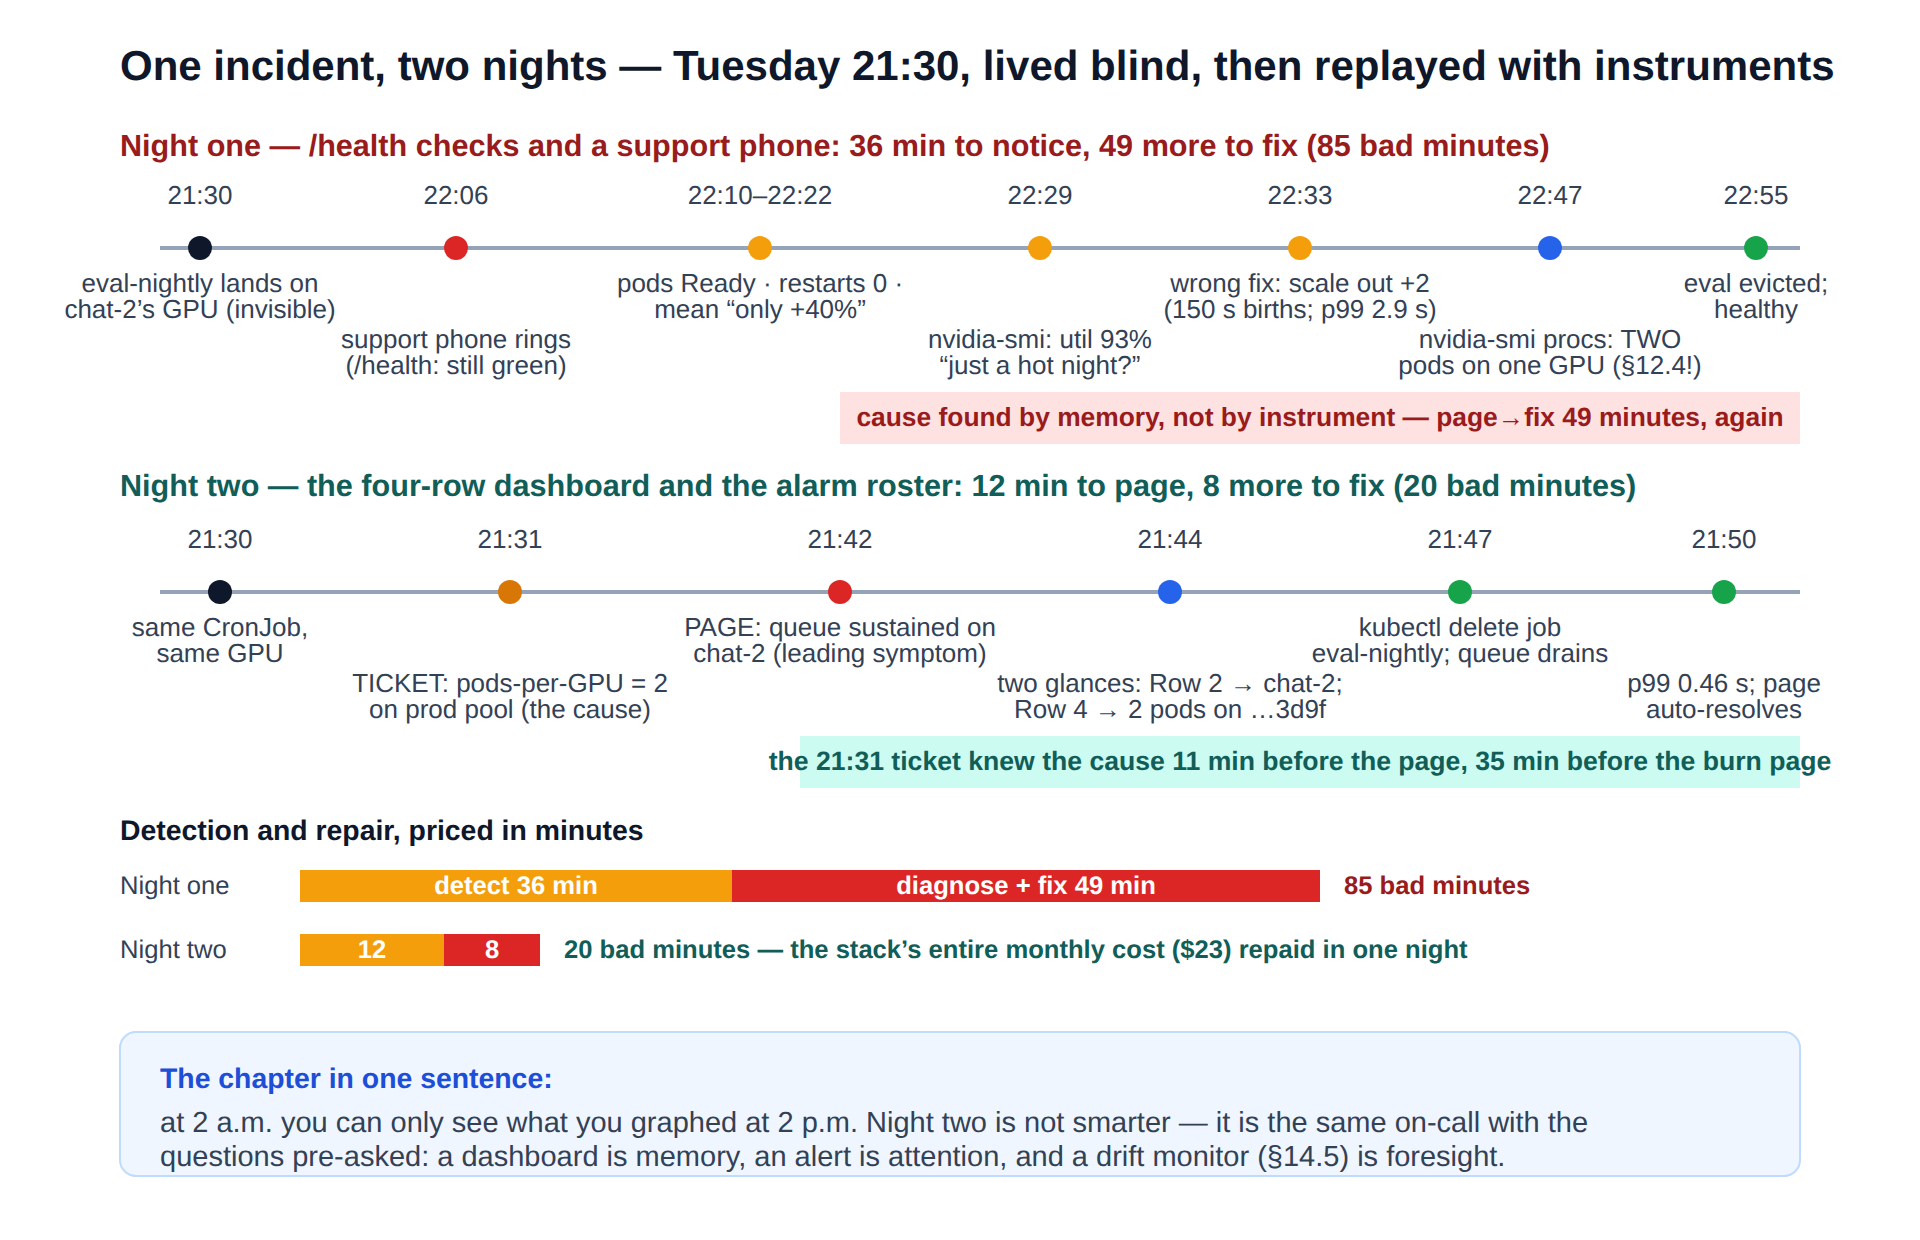
\includegraphics{figures/fig14-1_twonights.png}}\\[3pt]
  \figcaption{Figure 14-1  One incident, two nights. Night one: 36 minutes to notice via support, 49 more of tool-by-tool archaeology — 85 bad minutes, cause found by memory. Night two: cause ticketed at 21:31, symptom paged at 21:42, fixed by 21:50 — 20 bad minutes. The distance between the rows is this chapter.}
\end{tbbfigure}

\subsection*{November 14, 1969: the telemetry turned to garbage, and one controller had seen it before}

Thirty-six and a half seconds after Apollo 12 lifted off into a Florida rainstorm, lightning struck the Saturn V. Inside the capsule every warning light on the panel lit at once — fuel cells offline, buses undervolted — and in Houston the flight controllers’ screens dissolved into static-flecked nonsense numbers. The commander read his panel to the ground with professional calm and no idea what it meant. Sixteen seconds later a second strike made it worse. Mission control had under two minutes to decide whether to abort a Moon landing, and the room’s telemetry — the only view anyone had of a vehicle already beyond eyesight — was gibberish. Then a 24-year-old flight controller named \textbf{John Aaron} said one of the most famous sentences in spaceflight: \textit{“Flight, try SCE to Aux.”} Nobody else in the room — not the flight director, not the astronauts — knew what the switch was. A year earlier, during an unglamorous pad test, Aaron had watched telemetry decay into \textit{exactly that pattern} of nonsense, had traced it on his own time to an obscure box called the Signal Conditioning Equipment, and had learned that its auxiliary power mode cured it. Alan Bean, lunar module pilot, found the switch. Telemetry snapped back. The fuel cells were reset, the mission continued to the Moon, and Aaron acquired the nickname every operations engineer secretly wants: \textit{the steely-eyed missile man}.

Everything this chapter teaches is in that ninety seconds. \textbf{First: telemetry is designed, in advance, or it does not exist.} The Saturn V streamed thousands of channels to the ground because its engineers accepted that nobody would ever ssh into a rocket; your fleet crossed the same line the day it became four replicas on autoscaled nodes — Exhibit 14-A is what “walking out to look” costs at that scale. \textbf{Second: raw signal is not sight.} Houston had the data during those two minutes; what saved the mission was a \textit{recognized signature} — a pattern seen before, named, and attached to an action. That is precisely what a dashboard is: signatures drawn in advance, so that Tuesday’s on-call recognizes “one replica red, two pods one GPU” the way Aaron recognized SCE garble. \textbf{Third: the recognition was purchased in a drill.} Aaron had seen the failure in a \textit{test}, not a crisis — which is why this chapter’s lab ends by staging Exhibit 14-A against your own fleet, on purpose, with the dashboard open. NASA called it simulation; Chapter 13 called it break-it-twice; the SRE literature calls it a game day. The name matters less than the schedule. (Apollo has a second lesson waiting — a 1202 alarm, a hand-written cheat sheet, and the origin of every good paging policy — but it belongs to §14.4.)

\subsection*{Monitoring, observability, and the three pillars — the vocabulary, priced}

Terms, before the tooling. \textbf{Monitoring} is the practice of continuously collecting predefined signals and evaluating them against expectations — the questions you \textit{knew} to ask: is p99 under 500 ms, is the queue shallow, is the budget burning. \textbf{Observability} is the property of a system whose outward signals let you answer questions you did \textit{not} predefine — night two’s “why is one replica slow?” was nowhere in a runbook title, but queue-per-replica, decode-step-time, and pods-per-GPU could be \textit{composed} into the answer in two glances. You buy observability by exporting enough orthogonal, labeled signals; you practice monitoring by wiring the known ones to dashboards and alarms. The industry ships both through \textbf{three pillars}, and the honest way to choose among them is by cost shape (Figure 14-2). \textbf{Metrics} are numbers with labels, aggregated at the source — a counter of tokens, a gauge of queue depth, a histogram of TTFT. They cost almost nothing per event (an increment), survive any traffic volume unchanged, and are the only pillar cheap enough to evaluate \textit{continuously} — which is why alerts live here, and why this chapter does too. \textbf{Logs} are per-event records — the pod’s biography, indispensable for the one request that did something strange, linearly priced in volume (Chapter 5’s entourage promised you a log shipper; the lab installs one, structured JSON with a request\_id). \textbf{Traces} follow a single request across services with timing per hop — the microservice debugger’s pillar, sampled because they are the most expensive per event; the course keeps them thin (one OpenTelemetry paragraph in §14.2) because a four-hop serving path rarely needs what a 40-service checkout path does. One rule binds all three, paid for in Chapter 6’s coin: \textbf{telemetry ships off the pod, continuously} — a pod’s last minutes are exactly the minutes it will not live to narrate (the OOM kill of Chapter 3 left its evidence in cgroup counters and events, never in the app’s own log).

Chapter 5 gave you the sentence that separates this chapter from probes, and it is worth engraving: \textbf{probes are reflexes; monitoring is memory.} A liveness probe acts — restart on hang — and explains nothing; readiness acts — gate traffic — and explains nothing; both were green all Tuesday because the process was alive and answering. Monitoring explains and acts on nothing by itself: it is the system’s memory (what did the queue look like at 21:35?), its attention (the alert that turns memory into a phone buzz), and — with §14.5’s drift detection — its foresight (which direction is reality wandering?). A mature fleet needs both nervous systems: Chapter 5’s essay warned that reconciliation without observability is \textit{incident suppression}, self-healing that hides what it heals. This week the restart counters, OOM events, and endpoint gaps that Kubernetes has been quietly accumulating all become graphed, alertable lines — drift-correction \textit{frequency}, on a chart, is how you catch the limit that is sized one restart-per-90-seconds too small.

The map for the ninety minutes ahead. \textbf{§14.2} builds the signal layer — the three metric shapes, the exporter menagerie from node to DCGM to the engine’s own \code{/\allowbreak metrics} (Chapter 11’s lines, finally graphed), and the two PromQL incantations that make percentiles legal at fleet scale. \textbf{§14.3} assembles the \textbf{four-row dashboard} — promise, who, why, underneath — and then replays night two on it, panel by panel, paying §12.4’s debt in full. \textbf{§14.4} wires the \textbf{alarms}: the SLO sentence compiled into burn rates, the multiwindow policy that pages on fast burn and tickets slow burn, symptom-versus-cause routing, synthetic probes from outside every layer that can say no (Chapter 6’s door, watched at last), the dead man’s switch that watches the watcher — and the human loop of runbooks, on-call, and blameless postmortems. \textbf{§14.5} turns to the failure that never pages: \textbf{drift}, the slope your canary structurally cannot catch (Ch. 13’s cliffs-not-slopes, resolved), with a PSI you can compute by hand and sentinels the fleet already exports free. \textbf{§14.6} is the lab the syllabus promised — build the serving dashboard and its alarms — plus the part syllabi never promise: break it twice and let your own panels catch you. Mission control, then a mission.

\begin{calloutbox}{tbbpurple}{tbbpurplefill}
{\normalsize\bfseries\color{tbbpurple}Think About It}\par\vspace{3pt}
\begin{tbbitemize}
  \item Exhibit 14-A’s on-call ran five checks and each returned “fine.” For each of the five (probes, logs, mean latency, one pod’s /metrics, nvidia-smi util), name the question it ACTUALLY answers — and the question the SLO sentence needed answered. Which single panel from Figure 14-4 replaces all five?
  \item The 22:33 “wrong fix” (scale out to 6) genuinely improved p99 from 4.6 s to 2.9 s. Using Chapter 12’s arithmetic: why does adding replicas dilute but not cure a one-sick-replica incident — and what did the two extra replicas cost per hour while masking the diagnosis?
  \item John Aaron’s save required (a) telemetry that kept flowing during the anomaly, (b) a signature he had seen in a drill, (c) a switch that existed. Map all three onto night two — and identify which of the three your project fleet is currently missing for its most likely failure.
  \item Night two’s cause alert (21:31, ticket) preceded its symptom alert (21:42, page). Argue why the severities are assigned that way and not reversed — what happens to on-call life if every cause-shaped anomaly pages? (Hold your answer; §14.4 prices it with a hospital statistic.)
\end{tbbitemize}
\end{calloutbox}

\section{Metrics: Instrumenting the Fleet Honestly}

A \textbf{metric} is the smallest honest sentence a system can utter about itself: a \textit{name}, a set of \textit{labels}, a \textit{number}, and a \textit{time}. \code{vllm:num\_requests\_waiting\{pod="chat-2"\} 19 @21:41:30} — subject, qualifiers, verb, timestamp. Everything in this chapter is built from sentences of that shape, collected every fifteen seconds, kept for weeks, and queried in aggregate. Each distinct name-plus-label combination is a \textbf{time series}, and the first law of the trade is that you pay per \textit{series}, not per observation: a label with four values (the pods) multiplies a metric into four series, which is fine; a label with nine million values (a user or request id) multiplies it into nine million, which is a memory wall wearing a monitoring costume. The rule that keeps you solvent: \textbf{labels answer “which one?” from a bounded list} — pod, model, GPU UUID, route. Anything unbounded belongs in logs, where per-event storage is the design rather than the disaster. (The course fleet runs about 14,000 active series — Figure 14-2’s napkin — roughly a thousand samples per second and under two gigabytes per fifteen-day retention window. A single careless \code{user\_id} label would multiply that thousandfold.)

\begin{tbbfigure}
  \adjustbox{max width=0.94\linewidth,max totalheight=0.46\textheight}{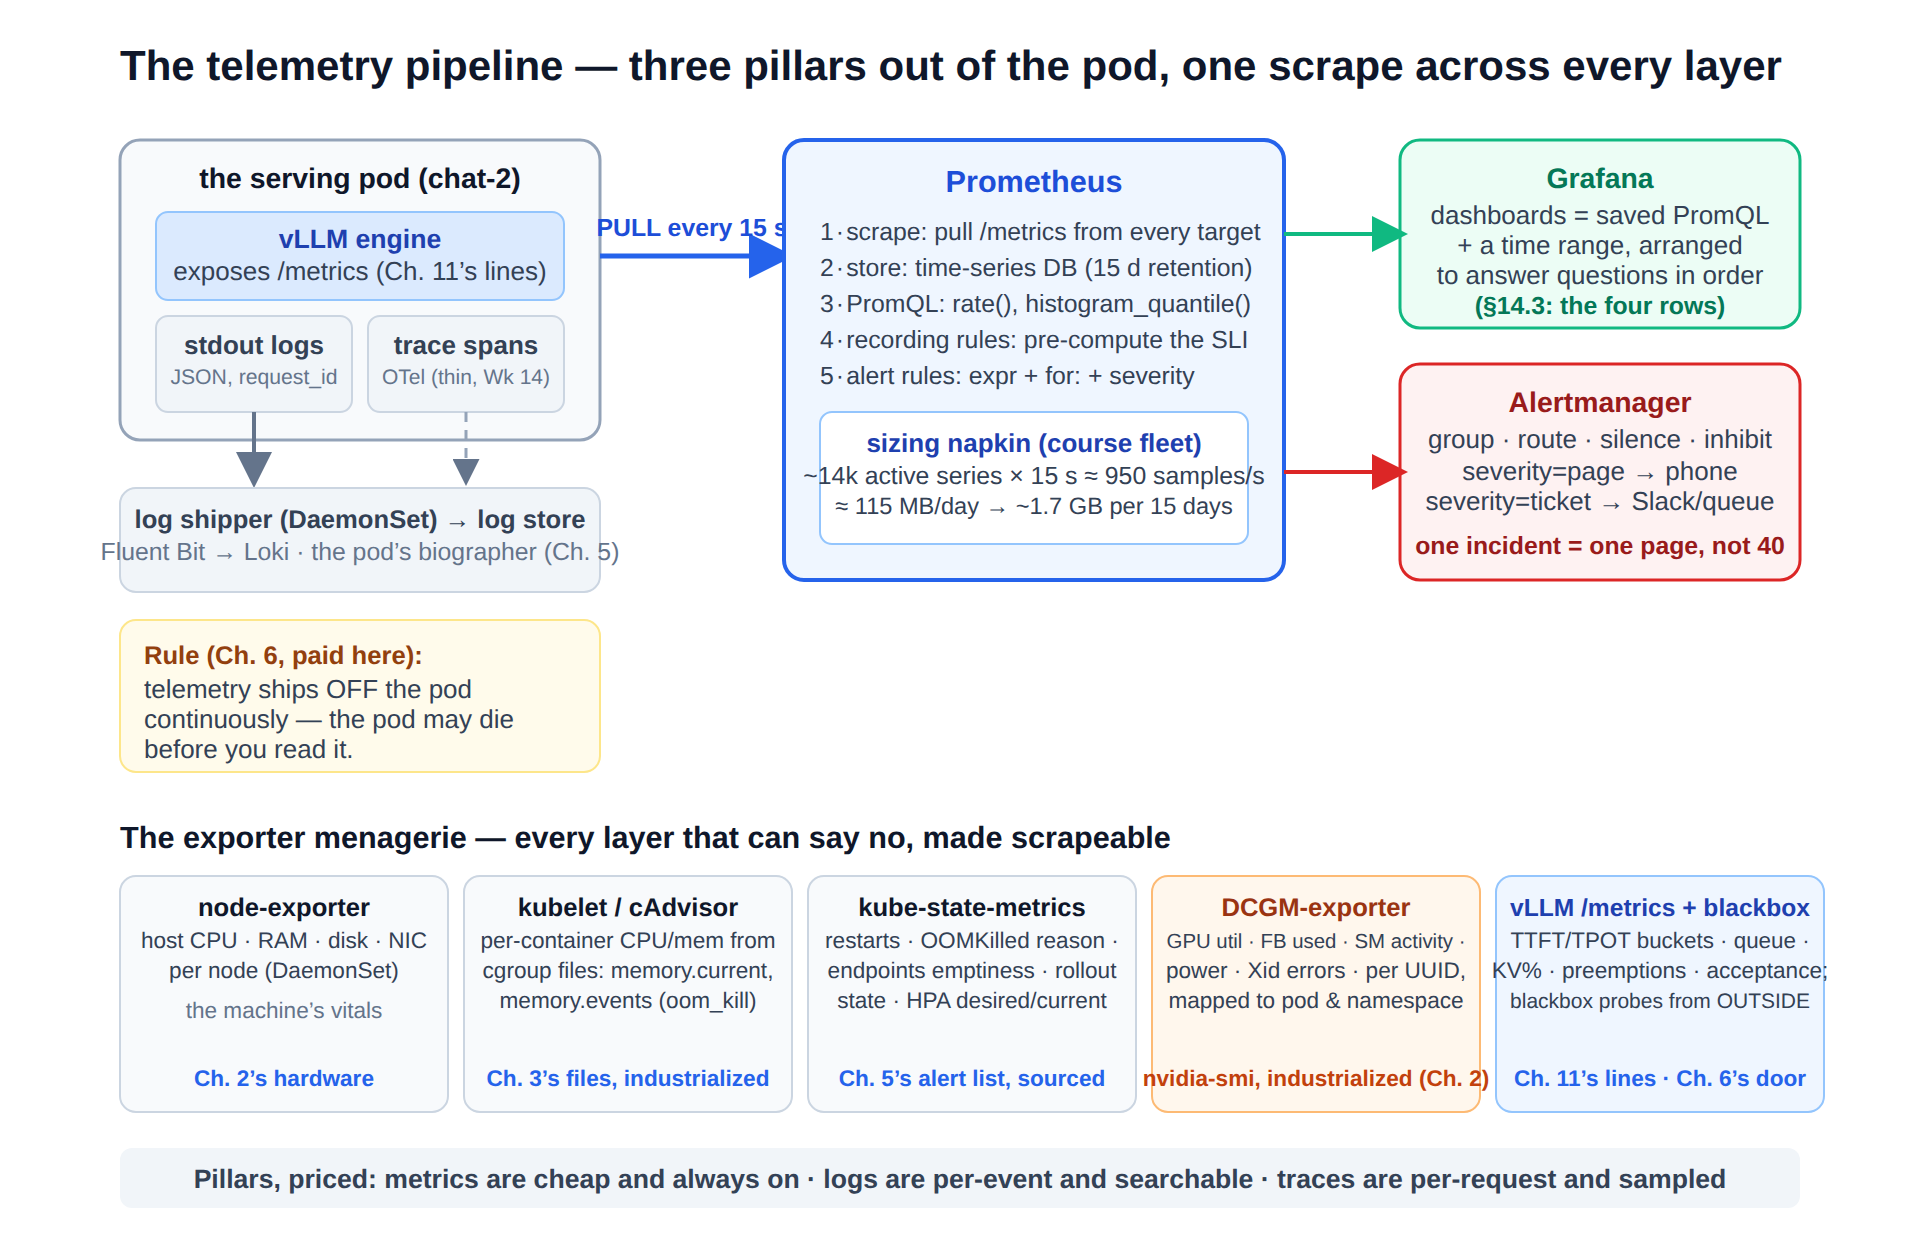
\includegraphics{figures/fig14-2_pipeline.png}}\\[3pt]
  \figcaption{Figure 14-2  The telemetry pipeline. Metrics are pulled off every layer by Prometheus and fan out to Grafana (questions) and Alertmanager (interruptions); logs ship via a DaemonSet the moment they are written; traces stay thin this course. Bottom: the exporter menagerie — six vantage points, one scrape loop, every layer that can say no made scrapeable.}
\end{tbbfigure}

\subsection*{Three shapes: counter, gauge, histogram — and why the third one runs this course}

Every metric you will ever export is one of three shapes, and choosing the wrong one is the beginner’s classic. A \textbf{counter} only climbs — tokens generated, preemptions since boot, requests completed. Its instantaneous value is trivia (1,841 preemptions... since \textit{when}?); its \textbf{rate of change} is the signal, which is why the query language’s workhorse is \code{rate(x[5m])}: the per-second slope over a window, computed restart-proof (a counter that resets to zero on pod rebirth is detected and bridged, one more reason to prefer counters over hand-rolled “requests this minute” gauges). A \textbf{gauge} is a value that goes both ways — queue depth, KV-cache fill, temperature. Gauges are read directly, aggregated with \code{max}/\code{avg} over pods or time, and are the natural shape for saturation signals. A \textbf{histogram} is the interesting one: a bank of \textit{cumulative buckets}, each a counter of observations at-or-below a threshold (\code{le="0.25"}, \code{le="0.5"}, ...), plus a running sum and count. It exists to solve exactly the problem Chapter 7 left you with: \textbf{percentiles cannot be averaged, and cannot be added} — ten replicas’ p99s do not combine into a fleet p99 by any arithmetic on the p99s themselves. Bucket \textit{counters}, though, add like any counters: sum the four replicas’ \code{le="0.5"} buckets and you have the fleet’s distribution, from which any quantile falls out. The histogram is Chapter 7’s grammar rule, shipped as a data structure.

Look at the shapes in the wild — the engine you have been running since Week 11 has been exporting all three the whole time:

\begin{terminalbox}
\begin{Verbatim}[breaklines=true,breakanywhere=true,fontsize=\small,formatcom=\color{tbbtermfg},codes=\tbbcodeactive]
$ curl -s chat-2:8000/metrics | grep -E 'vllm:' | head -14
vllm:num_requests_running{model="chat-v9"} 32.0     <- gauge: the seats,
vllm:num_requests_waiting{model="chat-v9"} 19.0        full (11.3); and THE
vllm:gpu_cache_usage_perc{model="chat-v9"} 0.96        alarm line (11.4)
vllm:num_preemptions_total{model="chat-v9"} 1841.0  <- counter: rate() it
vllm:spec_decode_draft_acceptance_rate{...} 0.74    <- gauge: 11.5's bet,
                                                       still paying
vllm:time_to_first_token_seconds_bucket{le="0.25"} 811021.0   <- histogram:
vllm:time_to_first_token_seconds_bucket{le="0.5"}  947210.0      cumulative
vllm:time_to_first_token_seconds_bucket{le="1.0"}  951003.0      buckets
vllm:time_to_first_token_seconds_bucket{le="+Inf"} 953882.0      (le = "at
vllm:time_to_first_token_seconds_count 953882.0                  or below")

$ curl -s gpu-node-2:9400/metrics | grep -E 'DCGM' | head -3
DCGM_FI_DEV_GPU_UTIL{UUID="GPU-...3d9f",pod="chat-2"} 93
DCGM_FI_DEV_FB_USED{UUID="GPU-...3d9f",pod="chat-2"} 22429
DCGM_FI_DEV_XID_ERRORS{UUID="GPU-...3d9f"} 0
\end{Verbatim}
\end{terminalbox}
\figcaption{Transcript 14-1  Two scrapes, annotated. The engine speaks all three shapes; note that 947,210 of 953,882 lifetime requests had TTFT ≤ 0.5 s — 99.3\%, the SLO’s own SLI, sitting in plain sight in two bucket counters. DCGM speaks for the silicon, labeled by GPU UUID and — via the device-plugin mapping — by pod, which is the join that solves Tuesday.}

Why \textbf{pull}? Prometheus scrapes targets rather than receiving pushes, and the choice is philosophy, not plumbing. Pulled targets are \textit{enumerated} — the server holds the list, discovered live from Kubernetes, so “which replicas exist” and “which stopped answering” are the same fact: every scrape writes an \code{up\{pod=...\}} series, and a pod that dies mid-incident leaves \code{up == 0} as its tombstone rather than a silence nobody notices (push systems discover absence only by modeling it). Pull also keeps instrumentation dumb — the engine just serves text over HTTP; no buffering, batching, or backpressure logic rides inside your latency-critical process. The cost is that Prometheus must be able to \textit{reach} targets, which inside one cluster is free. This design is inherited: Google’s internal \textbf{Borgmon} (born \textasciitilde{}2003 alongside Borg, Chapter 5’s ancestor) established the pattern — white-box \code{/\allowbreak varz} endpoints, a central puller, a query language over labeled series, alerts as queries — and when two ex-Google engineers, Matt T. Proud and Julius Volz, landed at SoundCloud in 2012 and found nothing comparable outside the fence, they rebuilt it in the open. \textbf{Prometheus} was open-sourced in 2015 and became the Cloud Native Computing Foundation’s second project ever — the first was Kubernetes, and the pairing is the industry admitting the two are halves of one design. \textbf{Grafana} arrived from the other direction: in 2014 Torkel Ödegaard forked a log-search UI (Kibana 3) into a general dashboard for time series. The stack you install in the lab is those two lineages, converged.

\subsection*{PromQL in four queries — including the two that settle Tuesday}

PromQL reads like set algebra over labeled series, and you can operate a fleet on perhaps a dozen idioms. The four below are this chapter’s load-bearing set — the middle two are Figure 14-3’s moral, run against the incident window:

\begin{terminalbox}
\begin{Verbatim}[breaklines=true,breakanywhere=true,fontsize=\small,formatcom=\color{tbbtermfg},codes=\tbbcodeactive]
# 1. the WRONG fleet p99 (tuesday, 21:44) -- averaging per-replica p99s:
> avg( job:vllm_ttft:p99_5m )
2.76                    # experienced by nobody (Figure 14-3)

# 2. the RIGHT fleet p99 -- merge bucket counters, THEN take the quantile:
> histogram_quantile(0.99,
    sum by (le) (rate(vllm:time_to_first_token_seconds_bucket[5m])))
9.08                    # the promise, actually broken

# 3. decompose: waiting or working? (Ch. 9's split, per replica)
> max by (pod) (vllm:num_requests_waiting)
{pod="chat-1"} 0   {pod="chat-2"} 19   {pod="chat-3"} 0   {pod="chat-4"} 0
> histogram_quantile(0.5, sum by (pod, le)
    (rate(vllm:time_per_output_token_seconds_bucket[5m])))
{pod="chat-2"} 0.150    # vs 0.070 fleet norm: decode itself is 2.1x slower

# 4. the SLI as a ratio -- the number 14.4 will set on fire:
> sum(rate(vllm:time_to_first_token_seconds_bucket{le="0.5"}[5m]))
  / sum(rate(vllm:time_to_first_token_seconds_count[5m]))
0.762                   # 76.2% good this window; target 0.990
\end{Verbatim}
\end{terminalbox}
\figcaption{Transcript 14-2  Four queries against the incident. Query 1 is the seductive wrong answer; query 2 is Chapter 7’s rule executed by machine; query 3 splits “waiting” from “working” — the diagnosis Chapter 9 promised would be half of this dashboard’s design; query 4 is the SLI ratio that §14.4 compiles into burn-rate pages.}

Read query 2’s anatomy once, inside out, and you own it: \code{rate(...bucket[5m])} turns each cumulative bucket counter into a per-second flow; \code{sum by (le)} adds those flows across replicas \textit{while preserving the bucket boundaries} — the only cross-replica aggregation that is mathematically legal for distributions; \code{histogram\_quantile(0.99, ...)} then walks the merged buckets to the 99th percentile, interpolating inside the winning bucket (which is why answers carry bucket-width granularity, and why the lab configures the engine’s buckets to put edges \textit{at} the SLO: a boundary at exactly 0.5 s makes the SLI ratio exact even while p99 estimates stay approximate). One more idiom deserves its name now: a \textbf{recording rule} is a query Prometheus re-evaluates on schedule and stores as a new series — \code{job:slo\_ttft\_good:ratio\_rate5m} for query 4, \code{job:vllm\_ttft:p99\_5m} per pod for the dashboard — so panels and alerts read precomputed answers instead of re-aggregating raw buckets at every refresh. Rules are YAML in the repo, PR-reviewed like everything since Chapter 13.

\subsection*{The exporter menagerie — six vantage points, and what each one is for}

Prometheus itself measures nothing; \textbf{exporters} hold the thermometers, and the menagerie in Figure 14-2’s bottom row is the course’s stack traversed one last time. \textbf{node-exporter} (a DaemonSet) speaks for the machine: CPU, memory, disk, network — Chapter 2’s hardware, as series. \textbf{cAdvisor}, built into the kubelet, speaks for every container by reading \textit{exactly the files you read by hand in Chapter 3}: cgroup \code{memory.current}, \code{memory.events}, CPU accounting. Two Chapter 3 lessons come due here. The honest-mounts footnote — a process inside a container that consults \code{/\allowbreak proc} sees the \textit{host’s} CPUs and memory, which is why naive in-container agents lie and why cAdvisor reads the cgroup tree from outside instead. And the tripwire — \code{memory.events} counts \code{high} and \code{oom\_kill} crossings, so the pre-wall warning phase you engineered with \code{memory.high} in the Chapter 3 lab is now a counter that Grafana can graph and §14.4 can ticket \textit{before} exit 137 (the exit code returns one final time, as a label value). \textbf{kube-state-metrics} speaks for the control plane’s \textit{intentions}: restart counts, \code{OOMKilled} as a last-termination reason, deployment replicas desired-versus-available, endpoint emptiness, HPA state — precisely the Chapter 5 alert list (“alert on drift-correction frequency, not just availability”), sourced. \textbf{DCGM-exporter} is \code{nvidia-smi} industrialized (Chapter 2’s promise): utilization, framebuffer, power, clocks, and Xid error codes per GPU UUID, joined to pod names through the device-plugin mapping — the join that made Tuesday a table lookup. It also carries the profiling family (\code{DCGM\_FI\_PROF\_SM\_ACTIVE}, tensor-pipe activity) that answers what “utilization” dodges — more on that lie in a moment. The \textbf{engine’s own /metrics} you have already met; add to it Chapter 9’s Triton counters for the classifier service, whose queue-time/compute-time split arrives pre-separated. And the \textbf{blackbox exporter} probes from \textit{outside} — an HTTP GET against the gateway’s public door, a TCP handshake, a streamed token — because Chapter 6 taught that every layer between user and pod can say no in its own vocabulary, and a fleet that only measures itself from inside will swear innocence while the load balancer’s health checks fail (the Transcript 6-11 lesson: the evidence lived outside the cluster). Synthetic checks are §14.4’s business; the exporter is how they become series.

Now the lie you met at 22:29. \code{DCGM\_FI\_DEV\_GPU\_UTIL} — the same number \code{nvidia-smi} prints — answers one question only: \textit{what fraction of recent time had at least one kernel, from anyone, resident on the device}. It is a \textbf{binary occupancy duty cycle}, not a measure of headroom, efficiency, or ownership. A memory-bound decode loop that keeps one thin kernel resident reads 90\%+ while using a tenth of the ALUs (Chapter 10’s roofline, restated as a dashboard trap); two tenants time-slicing a card \textit{both} push it toward 100\% while each gets half the work done; and nothing in the number says \textit{whose} kernels. Night one’s on-call read 93\% as “busy, therefore loaded, therefore normal” — three inferences, all unlicensed. The honest GPU questions and their honest sources: \textit{is the silicon earning its rent?} — \code{PROF\_SM\_ACTIVE} and tensor-pipe activity, against Chapter 10’s expectations; \textit{is memory the wall?} — \code{PROF\_DRAM\_ACTIVE} near saturation during decode is the memory wall, visible; \textit{is the card healthy?} — Xid errors, thermal, power; \textit{whose is it?} — the pods-per-UUID join, Row 4’s smoking gun. Utilization stays on the dashboard (it is a fine “something changed” line), but nothing pages on it, and the caption under it in the lab’s JSON reads, permanently: \code{busy ≠ yours ≠ efficient}.

Two framing acronyms organize any such menagerie, and interviewers love them. \textbf{RED} — Rate, Errors, Duration — is the \textit{service-side} view, one row per thing users call: requests per second, failure fraction, latency distribution. \textbf{USE} — Utilization, Saturation, Errors — is the \textit{resource-side} view, one row per thing services consume: how busy, how backed up, how broken. The mapping onto the course fleet is exact and worth internalizing: TTFT histograms are RED-Duration; \code{num\_requests\_waiting} is USE-Saturation for the seat pool — and saturation, not utilization, is the leading indicator everywhere in this book (the queue grows \textit{before} latency breaches, exactly as \code{memory.high} pressure precedes the OOM kill and Chapter 7’s knee precedes the hockey stick). KV-cache fill is USE-Utilization that is \textit{designed} to sit high — Chapter 11’s pinned-high-is-healthy, the gauge everyone new to the fleet misreads as an emergency. Preemption rate is USE-Saturation of the same pool expressed as evictions. The classifier’s queue-vs-compute split is RED-Duration decomposed by mechanism. Table 14-1 assembles the shopping list.

\begin{tbbtablewrap}
  \begin{tabular}{@{}>{\raggedright\arraybackslash}m{\dimexpr 0.2181\tbltextwidth-2\tabcolsep\relax} >{\raggedright\arraybackslash}m{\dimexpr 0.2766\tbltextwidth-2\tabcolsep\relax} >{\raggedright\arraybackslash}m{\dimexpr 0.1117\tbltextwidth-2\tabcolsep\relax} >{\raggedright\arraybackslash}m{\dimexpr 0.2606\tbltextwidth-2\tabcolsep\relax} >{\raggedright\arraybackslash}m{\dimexpr 0.1330\tbltextwidth-2\tabcolsep\relax}@{}}
  \arrayrulecolor{tbbnavy}\specialrule{1pt}{0pt}{0pt}
  \rowcolor{tbbtablehead}{\centering \bfseries\color{tbbnavy}Signal} & {\centering \bfseries\color{tbbnavy}Metric · source} & {\centering \bfseries\color{tbbnavy}Shape} & {\centering \bfseries\color{tbbnavy}The question it answers} & {\centering \bfseries\color{tbbnavy}Alarmed?} \\
  \arrayrulecolor{tbbnavy}\specialrule{0.7pt}{0pt}{2pt}
  {\textbf{TTFT distribution}} & {vllm:time\_to\_first\_token\_seconds · engine} & {histogram} & {is the promise kept? (Row 1; the SLI)} & {burn pair — page/ticket} \\
  \arrayrulecolor{tbbtableborder}\hline
  {\textbf{Decode pace}} & {vllm:time\_per\_output\_token\_seconds · engine} & {histogram} & {is generation itself slowing? (clause 2)} & {watch; ticket on trend} \\
  \arrayrulecolor{tbbtableborder}\hline
  {\textbf{Queue depth}} & {vllm:num\_requests\_waiting · engine} & {gauge} & {demand vs. seats — the leading symptom (Ch. 11)} & {PAGE (sustained)} \\
  \arrayrulecolor{tbbtableborder}\hline
  {\textbf{KV-cache fill}} & {vllm:gpu\_cache\_usage\_perc · engine} & {gauge} & {pool health — pinned-high is the design working} & {none (by design)} \\
  \arrayrulecolor{tbbtableborder}\hline
  {\textbf{Preemptions}} & {vllm:num\_preemptions\_total · engine} & {counter} & {is the pool thrashing? (KV pressure made visible)} & {ticket on rate} \\
  \arrayrulecolor{tbbtableborder}\hline
  {\textbf{Draft acceptance}} & {vllm:spec\_decode\_draft\_acceptance\_rate · engine} & {gauge} & {is speculation still paying? (drift sentinel, §14.5)} & {weekly review} \\
  \arrayrulecolor{tbbtableborder}\hline
  {\textbf{Restarts / OOM}} & {restarts\_total + OOMKilled reason · kube-state} & {counter} & {is self-healing hiding a leak? (Ch. 5, Ch. 3)} & {ticket; page if fleet-wide} \\
  \arrayrulecolor{tbbtableborder}\hline
  {\textbf{Endpoints ready}} & {endpoint address ready-count · kube-state} & {gauge} & {can the Service route to anyone? (Ch. 6’s 503)} & {PAGE at zero} \\
  \arrayrulecolor{tbbtableborder}\hline
  {\textbf{GPU health}} & {DCGM util / FB / Xid / PROF\_* · DCGM} & {mixed} & {what is the silicon doing — and whose is it?} & {Xid → ticket} \\
  \arrayrulecolor{tbbtableborder}\hline
  {\textbf{Door check}} & {probe\_success · blackbox} & {gauge} & {does it work from OUTSIDE? (Ch. 6’s door)} & {PAGE, 3 consecutive} \\
  \arrayrulecolor{tbbtableborder}\hline
  {\textbf{Fleet posture}} & {replicas desired vs. ready · kube-state/HPA} & {gauge} & {are pods chasing the wave? (Ch. 12)} & {ticket on stall} \\
  \arrayrulecolor{tbbnavy}\specialrule{1pt}{2pt}{0pt}
  \end{tabular}\par
  \figcaption{Table 14-1  The serving fleet’s metric shopping list. Two engine histograms, three engine gauges, one engine counter — then the platform’s memory (kube-state), the silicon’s vitals (DCGM), and the outside view (blackbox). The Alarmed column previews §14.4: two pages are symptoms, everything else files paper.}
\end{tbbtablewrap}

One honest word on the third pillar before leaving the signal layer. \textbf{Traces} — OpenTelemetry spans stitched across gateway, queue, and engine — earn their keep when a request’s time hides in the \textit{handoffs} between many services. The course path has three hops, and its handoff mystery (“waiting or working?”) is already answered by two metrics in query 3; so the course samples traces at 1\% with the OTel SDK’s default HTTP instrumentation and leaves deep span forestry to the microservice curricula. Similarly deferred: the \textbf{service mesh} (Ch. 5’s third sidecar, Ch. 6’s L7 cousin), which would hand you RED metrics for every hop \textit{for free} — genuinely its best sales pitch — at the price of a proxy in every pod and one more layer that retries (Chapter 6’s rule stands: one owner per concern; our gateway owns retries, so the mesh stays parked). What Week 14 does adopt from Chapter 5’s entourage prophecy: the metrics exporter and the log shipper, both installed in the lab; the mesh proxy remains “later,” possibly forever.

\begin{calloutbox}{tbbpurple}{tbbpurplefill}
{\normalsize\bfseries\color{tbbpurple}Think About It}\par\vspace{3pt}
\begin{tbbitemize}
  \item In Transcript 14-1, the lifetime buckets say 99.3\% of chat-2’s requests beat 0.5 s — yet chat-2 is the sick replica, mid-incident. Reconcile the two facts (hint: lifetime counters vs. rate() windows), and state the general rule about WHEN to look at raw counter values.
  \item Your teammate proposes labeling every engine metric with session\_id “so we can debug per-user.” Using the \textasciitilde{}14k-series napkin and \textasciitilde{}9.5M turns/month: estimate the series count after the change, name the failure mode, and give the correct home for per-request debugging (which pillar, which key).
  \item GPU util reads 41\% at 3 a.m. on the surviving night replicas. A cost-conscious PM asks “so we’re wasting 59\%?” Give the three-sentence answer that distinguishes duty-cycle from headroom, names the metric that would actually measure waste for a memory-bound decode fleet, and redirects the question to Chapter 12’s replica-hours arithmetic.
  \item Classify each Table 14-1 row as RED or USE, and notice the pattern in the Alarmed column: which method’s rows page, which file tickets — and why does that split reproduce §14.4’s symptom-vs-cause rule automatically?
\end{tbbitemize}
\end{calloutbox}

\section{Prometheus and Grafana: the Four-Row Dashboard, Live}

Installation is deliberately anticlimactic — the \textbf{kube-prometheus-stack} Helm chart lands Prometheus, Grafana, Alertmanager, node-exporter, and kube-state-metrics in one command (the lab’s step 1), pre-wired with the Kubernetes service discovery that makes pull work: Prometheus watches the API server, and any Service annotated for scraping becomes a target within a scrape interval. Teaching the stack about \textit{your} services takes one small custom resource each — a \textbf{ServiceMonitor} — plus the recording rules from §14.2, and both are ordinary YAML in the repository, shipped through Chapter 13’s pipeline like any other release artifact:

\begin{terminalbox}
\begin{Verbatim}[breaklines=true,breakanywhere=true,fontsize=\small,formatcom=\color{tbbtermfg},codes=\tbbcodeactive]
# monitoring/servicemonitor-chat.yaml -- "scrape every chat pod's :8000"
apiVersion: monitoring.coreos.com/v1
kind: ServiceMonitor
metadata: { name: chat-engine, labels: { release: kube-prometheus } }
spec:
  selector: { matchLabels: { app: chat } }
  endpoints: [ { port: http, path: /metrics, interval: 15s } ]
---
# monitoring/rules-slo.yaml -- the SLI, precomputed every 30 s
groups:
- name: slo.rules
  rules:
  - record: job:slo_ttft_good:ratio_rate5m
    expr: sum(rate(vllm:time_to_first_token_seconds_bucket{le="0.5"}[5m]))
          / sum(rate(vllm:time_to_first_token_seconds_count[5m]))

$ promtool check rules monitoring/rules-slo.yaml     # CI lane 1, extended
  SUCCESS: 1 rules found
$ kubectl -n monitoring get servicemonitors; open :9090/targets
  chat-engine ... 4/4 targets UP   dcgm ... 2/2 UP   blackbox ... 3/3 UP
\end{Verbatim}
\end{terminalbox}
\figcaption{Transcript 14-3  Wiring the stack: a ServiceMonitor per service, a recording rule for the SLI, promtool as the pipeline’s new gate (rules are release artifacts too — Chapter 13’s discipline did not stop at model weights), and the /targets page as the “is everything scraped?” roll call. up == 0 is itself an alertable series.}

Grafana’s mechanics you can learn in an afternoon — a \textbf{panel} is a PromQL query plus a visualization; a \textbf{dashboard} is panels plus a time range and template variables (\code{\$pod}, \code{\$model}); the whole thing serializes to JSON, and the lab stores that JSON \textit{in the repository}, because a dashboard is operational code: reviewed when it changes, versioned when it improves, recoverable when the Grafana pod is rescheduled (a dashboard that lives only in a UI is Chapter 13’s Friday deploy waiting to happen — nobody can say what “before” looked like). What cannot be learned from mechanics is \textbf{design}, and serving dashboards fail in a characteristic way: as a \textit{wall of everything} — forty panels, alphabetized, each individually true, collectively unreadable at 2 a.m. The design discipline this course teaches is the one in Figure 14-4: \textbf{one row per question, ordered exactly as the on-call’s runbook asks them.}

\begin{tbbfigure}
  \adjustbox{max width=0.94\linewidth,max totalheight=0.46\textheight}{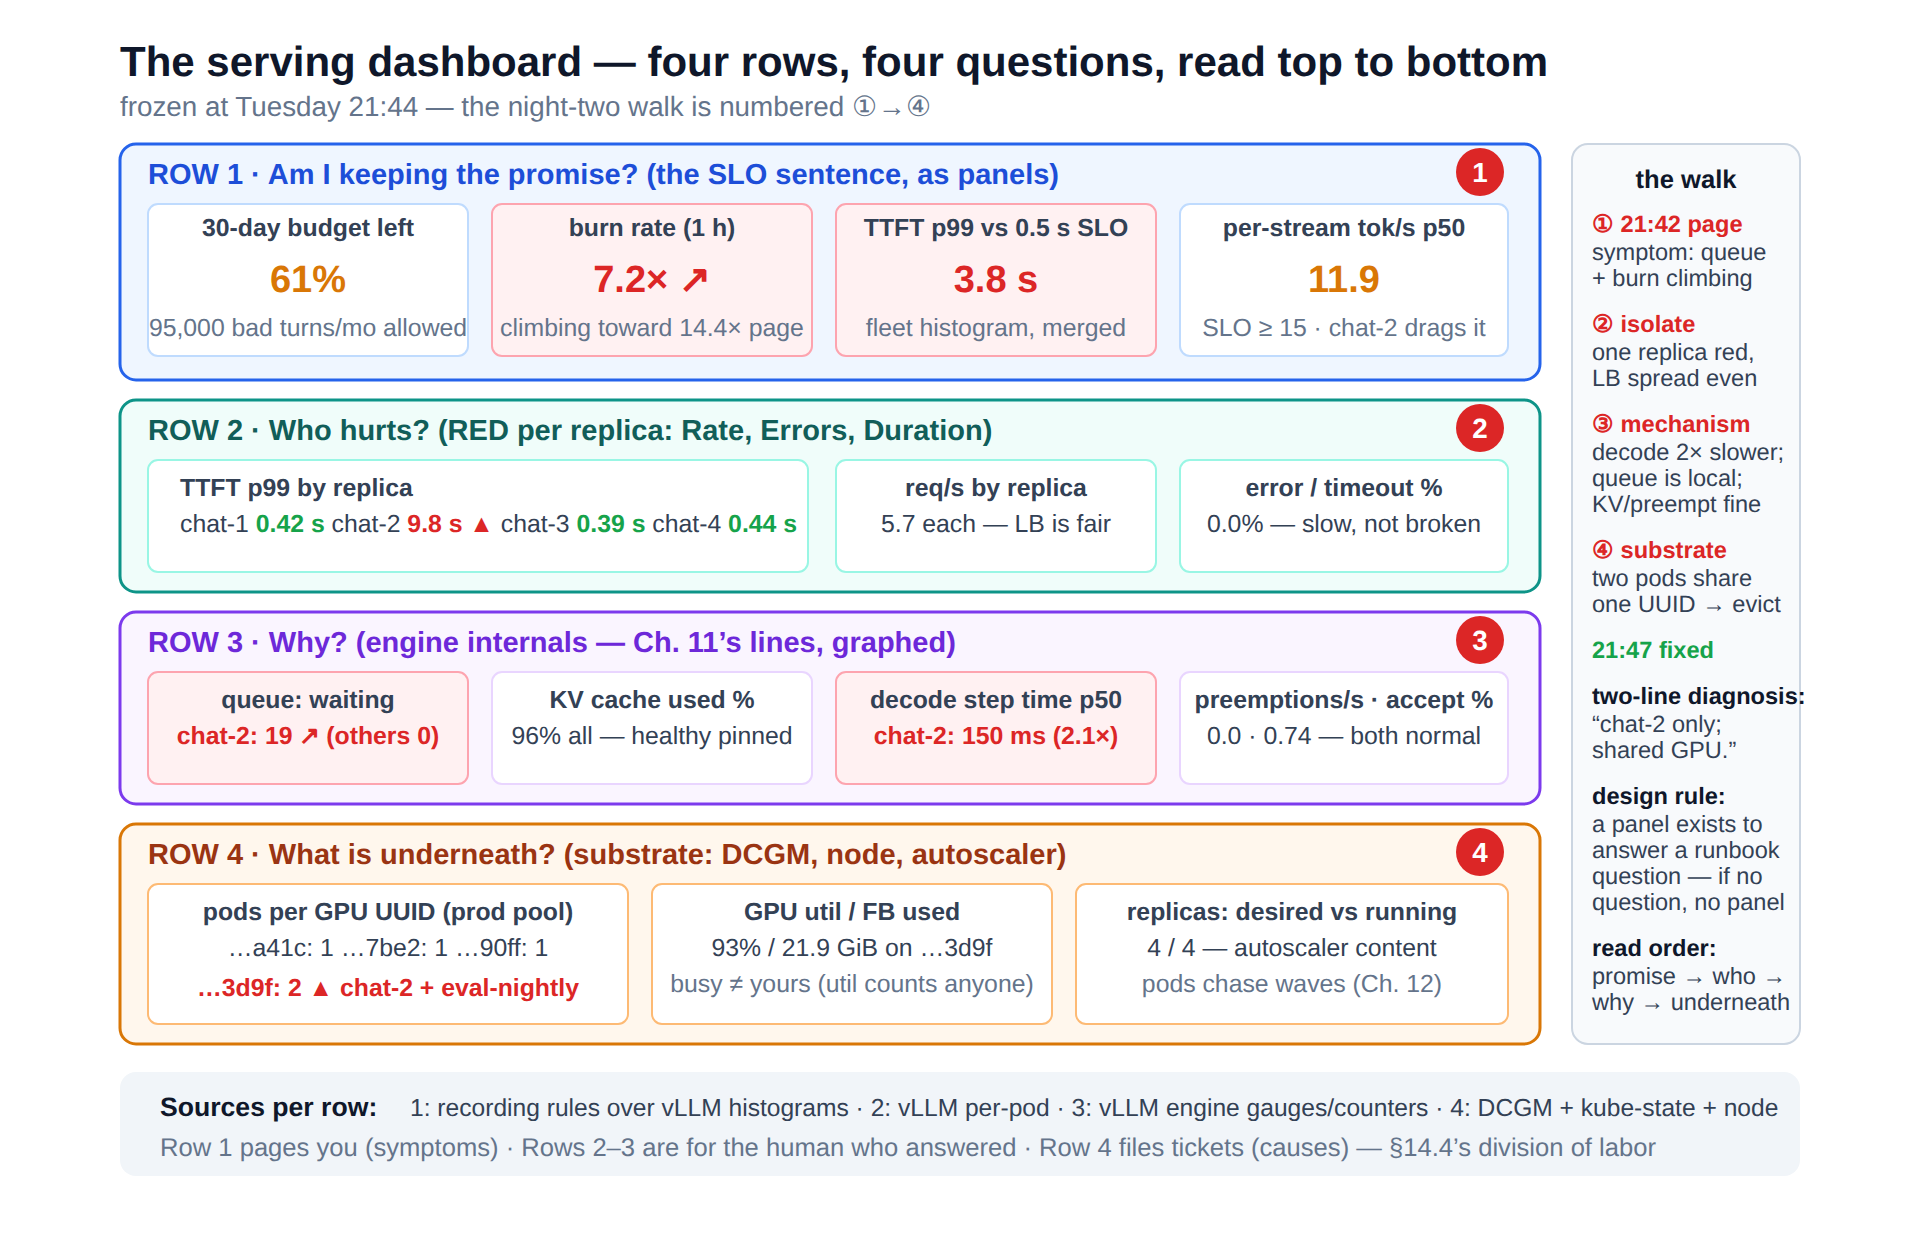
\includegraphics{figures/fig14-4_dashboard.png}}\\[3pt]
  \figcaption{Figure 14-4  The four-row serving dashboard, frozen at Tuesday 21:44. Row 1: am I keeping the promise? (the SLO sentence as panels — budget, burn, fleet p99, per-stream pace). Row 2: who hurts? (RED per replica). Row 3: why? (engine internals — queue, KV, decode pace, preemptions). Row 4: what is underneath? (DCGM per UUID, pods-per-GPU, autoscaler posture). The night-two walk is the numbered path ①→④.}
\end{tbbfigure}

\textbf{Row 1 answers “am I keeping the promise?” and nothing else.} Its panels are the SLO sentence translated term by term: the 30-day error-budget gauge (61\% remaining — the exact graph Chapter 7 promised would end arguments with product managers), the burn-rate line with the 14.4× page threshold drawn on it, fleet TTFT p99 computed the legal way (query 2, as a recording rule), and per-stream tokens/s p50 against the ≥15 clause. Everything here is a \textit{symptom} in §14.4’s vocabulary — user-visible promise-breakage — and Row 1 is therefore the only row wired to wake a human. \textbf{Row 2 answers “who hurts?”} — the same RED signals cut per replica and per route, because the first diagnostic fork in every capacity incident is \textit{everyone slow} (demand problem: knee, wave, storm) versus \textit{someone slow} (machine problem: this Tuesday). The panel that settles the fork in one glance is TTFT p99 by pod with the LB’s request-rate beside it: four fair shares of traffic, one unfair share of pain. \textbf{Row 3 answers “why?” in the engine’s own vocabulary} — Chapter 11’s lines, graphed at last: \code{num\_requests\_waiting} per pod (the leading indicator, the line Chapter 11 named THE alarm), KV-cache fill (pinned high across the fleet — healthy, annotated as such on the panel so 2 a.m. brains do not rediscover the misreading), decode-step pace (the mechanism detector: queue-with-slow-decode means the machine got slower; queue-with-normal-decode means demand outran seats), preemption rate and draft acceptance (pool pressure and speculation health). Row 3 is where Chapter 9’s promise — queue time and compute time arrive as separate counters, “half of Week 14’s dashboard design done for you” — is kept for the classifier and generalized for the LLM. \textbf{Row 4 answers “what is underneath?”} — DCGM per UUID with the pods-per-GPU join (Tuesday’s smoking gun: a table whose every prod row must read 1), framebuffer, Xid, node vitals, and the autoscaler’s desired-versus-running posture (pods chase waves; a wave the pods are \textit{not} chasing is its own incident class, Ch. 12’s stabilization windows visible as plateau lag).

Now watch the design pay for itself — the war story §12.4 scheduled, resolved on these four rows in real time, which is the demonstration Chapter 13’s next-chapter box promised you \textit{live}. \textbf{21:42, the page} (①): QueueSustained on chat-2, runbook link R2 in the page body, dashboard already filtered to the firing labels. Row 1 confirms the page is real — burn 7.2× and climbing, fleet p99 3.8 s — thirty seconds, no queries typed. \textbf{②, Row 2, the fork:} TTFT p99 by replica reads 0.42 / 9.8 / 0.39 / 0.44 — \textit{someone}, not everyone; and req/s per replica reads 5.7 across the board, so the LB is fair and the pain is intrinsic to chat-2. The everyone/someone fork just ate the entire “is it the knee? is it a storm? is it the deploy?” anxiety tree — there was no deploy, and this is not demand. \textbf{③, Row 3, the mechanism:} chat-2’s queue is 19 while its KV sits at the same 96\% as everyone (not a pool problem), preemptions flat (not thrash), but decode-step p50 is 150 ms against the fleet’s 70 — the \textit{machine itself} is slower, by 2.1×, which for a memory-bound loop (Ch. 10’s roofline, Ch. 11’s 20 ms floor) whispers: something else is drinking from this card’s memory bus. \textbf{④, Row 4, the substrate:} the pods-per-UUID table — GPU …3d9f: 2 (chat-2, eval-nightly-28471). There is the neighbor. \code{kubectl delete job eval-nightly}, a cordon note for the node’s stale time-slice ConfigMap, and by 21:50 the queue has drained, burn is under 1×, and the page resolves itself. Elapsed: eight minutes of human attention, two of them spent typing. The two-line diagnosis — \textit{“chat-2 only; shared GPU”} — is Chapter 6’s souvenir upgraded from aspiration to workflow, because the rows \textit{are} the two lines: Row 2 wrote the first, Row 4 wrote the second.

Three footnotes make the replay honest. First, the 21:31 \textbf{cause ticket} (pods-per-GPU = 2) had already named the culprit eleven minutes before the page — on night two the on-call could have read it in Slack before users felt anything; §14.4 explains why it files a ticket rather than paging even so (causes are legion, cheap, and often harmless; symptoms are few, expensive, and definitionally real — you page on the promise, and let causes annotate). Second, note what the dashboard did \textit{not} contain: a panel titled “time-slicing collisions.” Nobody predicted this failure; the rows answered it anyway, because each row answers a \textit{question} rather than enumerating known failures — that is observability doing its job, Aaron recognizing garble he had only ever seen in a drill. Third, the fix left \textbf{paper}: an incident note filed on the registry entry (Ch. 13’s runbook, whose WATCH step now reads “dashboard rows 1–2” instead of “curl /metrics and squint”), and — postmortem action, §14.4 — one new alert (the pods-per-GPU rule that was a lab exercise becomes fleet policy) plus one panel caption edited. A dashboard that does not change after an incident is a dashboard that learned nothing; the loop from incident to instrument is what makes monitoring \textit{compound}, and it is the loop the Chapter 10 lab quietly began when it made you store gate reports an incident reviewer could read.

\begin{calloutbox}{tbbred}{tbbxFEF2F2}
{\normalsize\bfseries\color{tbbx991B1B}Box 14-1  The seven deadly sins of serving dashboards}\par\vspace{3pt}
\begin{tbbitemize}
  \item \textbf{Means on the marquee.} A mean headline over a skewed distribution is Exhibit 14-A’s “+40\%, users exaggerate.” Percentiles or histograms, always; the mean describes nobody.
  \item \textbf{Averaged percentiles.} avg() over per-replica p99s produced 2.76 s against a true 9.08 s. Merge buckets (sum by le), then quantile — no exceptions, including in ad-hoc queries under pressure.
  \item \textbf{Utilization read as headroom.} GPU util is occupancy duty-cycle: busy ≠ yours ≠ efficient. Saturation signals (queue, preemptions, DRAM activity) carry the meaning util pretends to.
  \item \textbf{No SLO line on the graph.} A p99 panel without the 0.5 s threshold drawn on it outsources the judgment to memory at 2 a.m. Draw the promise on every panel that measures it.
  \item \textbf{Alerts without runbooks (or panels without questions).} Every page links a runbook; every runbook step names a row; every panel exists because a runbook asks its question. Anything else is decoration.
  \item \textbf{The wall of everything.} Forty alphabetized panels answer nothing. Four rows, ordered promise → who → why → underneath, read top-down in under a minute — one dashboard per audience, not one panel per metric.
  \item \textbf{Unversioned dashboards.} JSON in the repo, reviewed like code, or your instrument panel is one pod reschedule from amnesia — the Friday deploy, monitoring edition.
\end{tbbitemize}
\end{calloutbox}

\begin{calloutbox}{tbbpurple}{tbbpurplefill}
{\normalsize\bfseries\color{tbbpurple}Think About It}\par\vspace{3pt}
\begin{tbbitemize}
  \item Reconstruct night two with ROW 2 missing: which questions become expensive, in what order does the on-call now check things, and how many of night one’s 49 minutes return? (This is the graded question behind “which row would you cut?” — the answer is an argument, not a preference.)
  \item The fleet p99 panel (query 2) and the SLI ratio panel (query 4) can disagree: construct a 5-minute window where p99 ≤ 0.5 s but the SLI ratio is below target, and one where the reverse holds. Which belongs on Row 1 wired to the pager, and why does §14.4 choose the ratio?
  \item Your teammate wants a fifth row: “business — sign-ups, tokens sold, revenue/M.” Make the case for and against putting it on THIS dashboard (audience, refresh cadence, who acts on it), and name where Chapter 12’s unit-economics line actually belongs.
  \item The pods-per-GPU panel needed a join between DCGM (UUID-labeled) and the device plugin’s pod mapping. If your cluster’s DCGM exporter lacked the pod label, design the two-step manual join the on-call performs at 21:44 — and estimate what it costs in minutes against night one’s 49.
\end{tbbitemize}
\end{calloutbox}

\section{Alerting: Pages, Burn Rates, and the Art of Not Crying Wolf}

A dashboard is memory; an \textbf{alert} is attention — the machinery that decides, on your behalf and at any hour, that a human must stop sleeping now. That decision deserves the same engineering rigor as the serving path, and history’s best case study happened 250,000 miles from the nearest pager. July 20, 1969: five minutes into the first Moon landing’s powered descent, the guidance computer flashed \textbf{1202} — an alarm code exactly nobody in the capsule had memorized. Fuel burning, surface approaching, and the crew’s displays offering four digits of pure ambiguity. The GO call came from the ground in under thirty seconds, and it came off a \textbf{hand-written cheat sheet}. Three weeks earlier, in a training simulation, the control team had seen a sister alarm (1201), panicked, and called an abort — \textit{wrongly}, it turned out, and the simulation supervisor made sure the lesson stung. A 24-year-old backroom engineer named Jack Garman went home and wrote out every program alarm code by hand, with, next to each, the condition under which it mattered. His note for the executive-overflow family said, in effect: \textit{if it does not recur too often, and guidance keeps flying, GO.} When 1202 fired for real, Steve Bales in the front room relayed Garman’s verdict, Armstrong kept descending, and the alarm — the computer announcing it was overloaded but \textit{shedding low-priority work by design} (Margaret Hamilton’s priority executive: Chapter 9’s shed-load principle, running on 4 KB of RAM) — fired three more times without consequence.

Every rule this section teaches is in that story. The alarm’s meaning was decided \textbf{in advance, in writing} — a runbook, born from a \textit{failed drill} (your lab’s break-it-twice has a forty-year pedigree). The verdict keyed on \textbf{rate and persistence, not existence} — “doesn’t recur too often” is \code{for: 5m} and a rate threshold, 1969 edition; a single spike of anything is almost never a page. The system under alarm was \textbf{degrading gracefully by design} — some alarms describe the design \textit{working} (KV cache pinned high; the executive shedding tasks), and paging on them trains humans to ignore pages. And the human cost of getting this wrong has a body count outside spaceflight: hospital telemetry wards, the densest alarm environments ever built, taught the industry the term \textbf{alarm fatigue}. The Joint Commission’s 2013 sentinel-event alert counted 98 alarm-related incidents in three and a half years — 80 of them fatal — and cited studies finding that \textbf{85–99\% of clinical alarms require no intervention at all}: nurses drowning in beeps learn, rationally, that beeps mean nothing, and then one of them does. The engineering translation is brutal and freeing: every alert that is not \textit{actionable, urgent, and real} actively trains your team to miss the one that is. A page is not information; it is a command to wake up. Issue few.

\subsection*{Symptoms page; causes ticket}

The discipline that operationalizes “issue few” is a two-word routing rule, canonized in Rob Ewaschuk’s \textit{My Philosophy on Alerting} and the SRE book after it: \textbf{page on symptoms, ticket on causes.} A \textit{symptom} is user-visible promise-breakage — the SLI bleeding, the queue drowning requests, the door refusing from outside. A \textit{cause} is any condition that might eventually produce one — a leaking replica, a stale ConfigMap, two pods on one GPU. The asymmetry that justifies the rule: symptoms are \textbf{few, definitionally real, and complete} (any user-hurting failure, including ones you never imagined, must eventually surface in the SLI — Tuesday’s time-slice collision was invented after your alert rules were written, and the queue page caught it anyway), while causes are \textbf{legion, cheap, and often harmless} (the same duplicate-pods condition on the \textit{dev} pool is Tuesday-normal; time-slicing was §12.4’s honest recommendation there). Page on causes and you inherit the hospital ward: a rotation numbed by 3 a.m. non-events. So Tuesday’s pods-per-GPU alert filed a \textbf{ticket} — visible in Slack at 21:31, priceless \textit{once a symptom made it relevant}, silent on the pager. The night’s one page was the queue: a leading symptom (users were already waiting in it) that beat the lagging one (the burn-rate page, 24 minutes behind it) — the same tripwire-before-wall pattern as Chapter 3’s memory.high, and the reason Table 14-1 put its only sustained-gauge PAGE on \code{num\_requests\_waiting}, the line Chapter 11 appointed to exactly this job.

\subsection*{Compiling the SLO sentence: error budgets and burn rates, worked}

Chapter 13 promised that this chapter would make “pages fire on burn rates rather than vibes,” so here is the compilation, end to end, of the course SLO’s availability clause. The Week 11 contract says \textbf{TTFT p99 ≤ 500 ms} — which is the same sentence as: \textit{at least 99\% of turns receive their first token within 0.5 s}. Restated as a ratio it becomes an \textbf{SLI} (Transcript 14-2, query 4), and the 1\% complement becomes the \textbf{error budget}: at the fleet’s \textasciitilde{}9.5 million turns a month (2.0 B served tokens at the \textasciitilde{}211-token mean answer), the promise grants \textbf{\textasciitilde{}95,000 bad turns per 30 days} — a resource, exactly as Chapter 7 framed the 43 minutes of a time-based 99.9\% (note the unit change: request-based budgets count turns, not minutes, which is why they stay meaningful across the diurnal wave — a bad \textit{minute} at 3 a.m. spends almost nothing; a bad minute at 21:30 spends a fortune, and that is the correct pricing of user pain). The \textbf{burn rate} is spend speed: burn = (bad-turn fraction) ÷ (1 − SLO). Burning at 1× exhausts the budget in exactly 30 days — the break-even pace. Tuesday at 21:44, with chat-2 drowning a quarter of arrivals, the bad fraction was \textasciitilde{}24\%, so burn ≈ 24×: a month of budget in 30 hours. Figure 14-5 draws the tank and its drains.

\begin{tbbfigure}
  \adjustbox{max width=0.94\linewidth,max totalheight=0.46\textheight}{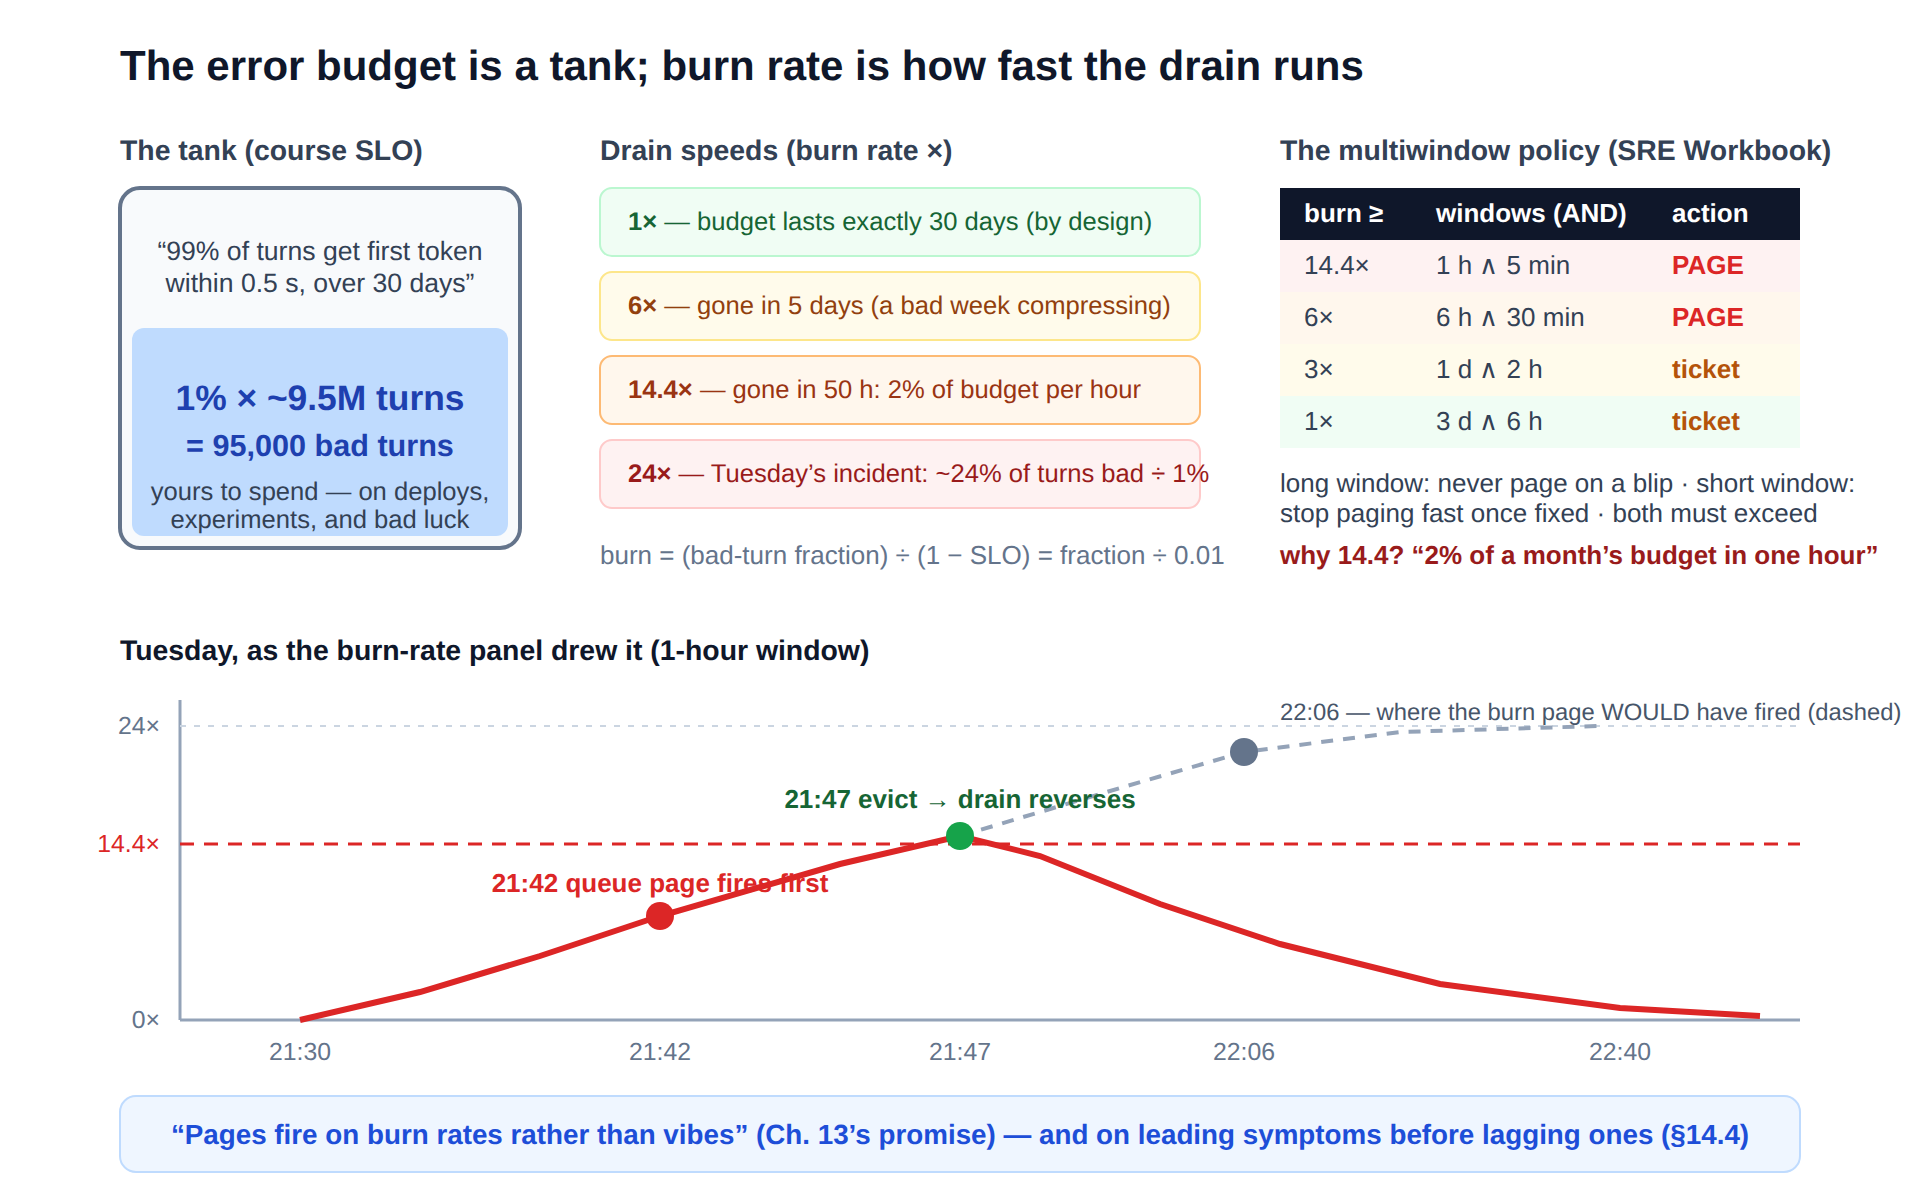
\includegraphics{figures/fig14-5_burnrate.png}}\\[3pt]
  \figcaption{Figure 14-5  The budget tank (95,000 bad turns), four drain speeds, the multiwindow policy, and Tuesday as the 1-hour burn panel drew it: the queue page beat the burn page by 24 minutes; the dashed line is where the burn page would have fired unmitigated (22:06).}
\end{tbbfigure}

Alerting on burn is a windows game, and the standard policy — the SRE Workbook’s, adopted wholesale by the lab — uses \textbf{paired windows} per severity: page when burn ≥ \textbf{14.4× over both 1 h and 5 min} (that pace spends 2\% of the month’s budget per hour); page at \textbf{6× over 6 h and 30 min} (5\% per six hours — the slow bleed a fast rule misses); ticket at \textbf{3× over a day} and at \textbf{1× over three days} (trajectory warnings that belong in daylight). Each pairing encodes one temperament trade: the \textbf{long window is skepticism} — a 90-second blip, whatever its depth, cannot move a 1-hour average past 14.4×, so blips never page (Apollo’s “doesn’t recur too often,” as arithmetic); the \textbf{short window is forgiveness} — once the incident ends, the 5-minute average collapses immediately and the page resolves, instead of echoing for the rest of the hour while the long window drains. The honest cost of skepticism is latency: at Tuesday’s 24× burn, the 1-hour average needed \textasciitilde{}35 minutes to cross 14.4× (24 × 35/60 = 14) — which is precisely why the roster does not rely on burn alone. Burn pages are the \textbf{completeness guarantee} (every user-visible failure, known or novel, eventually trips them); the queue page is the \textbf{fast path} for the failure mode this fleet actually has (capacity-shaped pain arrives queue-first, Chapter 7’s knee and Chapter 11’s admission line). Fast paths are allowed. Only symptoms get them.

\begin{terminalbox}
\begin{Verbatim}[breaklines=true,breakanywhere=true,fontsize=\small,formatcom=\color{tbbtermfg},codes=\tbbcodeactive]
# monitoring/rules-alerts.yaml (excerpt) -- the roster's teeth
- alert: SLOBurnFast                              # completeness guarantee
  expr: >
    (1 - job:slo_ttft_good:ratio_rate1h) / 0.01 > 14.4
    and (1 - job:slo_ttft_good:ratio_rate5m) / 0.01 > 14.4
  labels: { severity: page }
  annotations: { runbook: runbooks/R1-slo-burn.md }

- alert: QueueSustained                           # fast path (symptom)
  expr: avg_over_time(vllm:num_requests_waiting[5m]) > 8
  for: 5m
  labels: { severity: page }
  annotations: { runbook: runbooks/R2-queue.md, dashboard: row 3 }

- alert: DuplicatePodsOnProdGPU                   # cause (tuesday's vaccine)
  expr: count by (UUID) (DCGM_FI_DEV_GPU_UTIL{pool="prod"}) > 1
  for: 2m
  labels: { severity: ticket }

- alert: Watchdog                                 # dead man's switch
  expr: vector(1)                                 # fires ALWAYS, on purpose
  labels: { severity: heartbeat }

# alertmanager.yaml (excerpt) -- routing, grouping, silence
route:
  group_by: [alertname, model]      # one incident = one page, not 40
  routes:
  - match: { severity: page }    receiver: oncall-phone
  - match: { severity: ticket }  receiver: slack-serving-alerts
  - match: { severity: heartbeat } receiver: deadman-external
$ amtool silence add alertname=QueueSustained --duration=2h \
    --comment "drill A in progress (lab 14)"      # planned breakage, quiet
\end{Verbatim}
\end{terminalbox}
\figcaption{Transcript 14-4  Alerts are queries with severities; routing is policy. Note the shapes: the burn pair reads recording rules; the queue page needs sustain (for: 5m); the cause rule tickets; the Watchdog fires forever so that its SILENCE — detected by an external receiver expecting the heartbeat — means the monitoring stack itself is down. Who watches the watchers: a switch that a dead man releases.}

\begin{tbbtablewrap}
  \begin{tabular}{@{}>{\raggedright\arraybackslash}m{\dimexpr 0.2500\tbltextwidth-2\tabcolsep\relax} >{\raggedright\arraybackslash}m{\dimexpr 0.3085\tbltextwidth-2\tabcolsep\relax} >{\raggedright\arraybackslash}m{\dimexpr 0.1223\tbltextwidth-2\tabcolsep\relax} >{\raggedright\arraybackslash}m{\dimexpr 0.3191\tbltextwidth-2\tabcolsep\relax}@{}}
  \arrayrulecolor{tbbnavy}\specialrule{1pt}{0pt}{0pt}
  \rowcolor{tbbtablehead}{\centering \bfseries\color{tbbnavy}Alert} & {\centering \bfseries\color{tbbnavy}Condition (sketch)} & {\centering \bfseries\color{tbbnavy}Severity} & {\centering \bfseries\color{tbbnavy}Why it exists · lineage} \\
  \arrayrulecolor{tbbnavy}\specialrule{0.7pt}{0pt}{2pt}
  {\textbf{SLOBurnFast}} & {burn ≥ 14.4× over 1 h ∧ 5 m} & {PAGE} & {the promise, bleeding fast — catches even unimagined failures (Ch. 7 → here)} \\
  \arrayrulecolor{tbbtableborder}\hline
  {\textbf{SLOBurnSlow}} & {burn ≥ 3× over 1 d (and 1×/3 d)} & {ticket} & {trajectory warning; spend the budget on purpose, in daylight} \\
  \arrayrulecolor{tbbtableborder}\hline
  {\textbf{QueueSustained}} & {waiting > 8 for 5 m on any pod} & {PAGE} & {the fast path — capacity pain arrives queue-first (Ch. 11’s alarm line)} \\
  \arrayrulecolor{tbbtableborder}\hline
  {\textbf{EndpointsEmpty}} & {ready addresses = 0 on chat Service} & {PAGE} & {nobody to route to = every user sees Ch. 6’s 503, now} \\
  \arrayrulecolor{tbbtableborder}\hline
  {\textbf{ProbeFail}} & {probe\_success = 0, 3 consecutive, any probe} & {PAGE} & {the door refused from outside — layers the fleet cannot see (Ch. 6)} \\
  \arrayrulecolor{tbbtableborder}\hline
  {\textbf{PreemptionSurge}} & {rate(preemptions) > 0.5/s for 10 m} & {ticket} & {KV pool thrashing; often prompt-length drift arriving (§14.5)} \\
  \arrayrulecolor{tbbtableborder}\hline
  {\textbf{RestartsOOM}} & {Δrestarts ≥ 3/h, or OOMKilled seen} & {ticket → page if fleet-wide} & {self-healing hiding a leak (Ch. 5’s list; Ch. 3’s exit 137)} \\
  \arrayrulecolor{tbbtableborder}\hline
  {\textbf{DuplicatePodsOnProdGPU}} & {pods per prod UUID > 1 for 2 m} & {ticket} & {Tuesday’s vaccine — a cause, so it annotates rather than wakes} \\
  \arrayrulecolor{tbbtableborder}\hline
  {\textbf{Watchdog}} & {vector(1) — always firing} & {heartbeat} & {dead man’s switch: its silence pages, via a receiver outside the cluster} \\
  \arrayrulecolor{tbbnavy}\specialrule{1pt}{2pt}{0pt}
  \end{tabular}\par
  \figcaption{Table 14-2  The alarm roster. Four pages — all symptoms, all with runbooks; four tickets — all causes; one heartbeat. Contrast the shape with the hospital ward’s hundreds: a rotation that trusts its pager is the deliverable.}
\end{tbbtablewrap}

\subsection*{Synthetic probes: standing outside every layer that can say no}

Everything above watches the fleet from inside its own walls, and Chapter 6 spent a whole lab proving how much that view misses: the LB health-checking a path nobody implemented, TLS expiring, the perimeter’s timeout stricter than yours — failures where kubectl swears innocence while customers see 503, because the evidence lives in a console \textit{outside the cluster}. The \textbf{synthetic probe} is monitoring’s answer, and the Chapter 6 exercise that asked you to design three of them gets its official solution here. Probe one, \textbf{the door}: an HTTPS \code{GET /\allowbreak v1/\allowbreak models} against the public gateway URL from the blackbox exporter, every 30 s — it exercises DNS, TLS, LB target health, and routing, and \textit{must run from outside the LB} or it validates nothing (a probe that shares fate with the thing it checks is a mirror, not a witness; the truly paranoid run it from a second region). Probe two, \textbf{the answer}: a one-token completion with a 10 s timeout every minute — it exercises the full path including admission and engine, and catches the 504/hang class the door probe sails past. Probe three, \textbf{the stream}: a short streamed completion that must receive its first token ≤ 2 s and its final chunk intact, every 5 min — the stream-cut detector, standing outside the \textit{idle-timeout} layer that Chapter 6’s Table 6-3 blamed for mid-answer silence. Three probes, three layers, each outside the layer it indicts; \code{probe\_success} pages on three consecutive failures (existence would page on every network sneeze — Garman again). Together they close the course’s oldest observability gap: the uptime checker in Exhibit 14-A was green all night \textit{because it was probe one alone} — aliveness of the door, saying nothing about the queue behind it. Synthetics complete the promise made when the course first sent you to the LB’s target-health console: \textbf{observability must cover every layer that can say no — from a vantage point that layer cannot suborn.}

\subsection*{The human half: on-call, runbooks, postmortems — and what the numbers buy}

A page lands on a person, and the machinery around that person is as designed as the PromQL. The \textbf{on-call rotation} carries the pager in shifts with an explicit contract: acknowledge in minutes, escalate freely, hand off in writing — sustainable precisely because Table 14-2 pages perhaps monthly, not nightly. The \textbf{page carries its runbook} (Ch. 13’s template, now with teeth): SYMPTOM → the dashboard row that answers it → safe mitigations in order of reversibility → the escalation line — and the runbook’s WATCH step, which Chapter 13 could only point at \code{/\allowbreak metrics} and a script, now reads \textit{“rows 1–2, burn and per-replica”}. After resolution comes the practice the industry adopted from aviation and John Allspaw’s crusade: the \textbf{blameless postmortem}. Blameless is not politeness; it is epistemics — Chapter 13 already made the argument (individuals err at a constant rate; systems set the price), and a postmortem that ends in a name learns nothing, while one that ends in a \textit{mechanism} produces action items. Tuesday’s produced three, filed within a day: the pods-per-GPU rule promoted from lab exercise to fleet policy (a cause alert born, correctly, as a ticket); the stale time-slice ConfigMap given an owner and an expiry check in CI; and one dashboard caption edited (“busy ≠ yours”). The write-up itself was \textbf{filed on the registry entry} for v9-int4 — the Chapter 10 lab told you an incident reviewer would someday read your stored gate reports, and this is that reader, closing the file. That loop — incident → instrument — is what makes monitoring \textit{compound}: every fire leaves behind a smoke detector.

Two numbers grade the whole apparatus, and they close accounts this book opened weeks ago. \textbf{MTTD} (mean time to detect: incident start → humans know) and \textbf{MTTR} (mean time to restore: incident start → users fine) — Figure 14-1’s bars, 36+49 versus 12+8. MTTR is DORA’s fourth key (Ch. 13 priced the other three), and the course’s deployment story ends with all four keys instrumented rather than estimated. These distributions are also \textit{design inputs}: Chapter 13’s essay asked what data would tune the blue/green warm-standby hour, and the answer is now on a dashboard — if your MTTD for deploy-shaped regressions is 12 minutes, an hour of double-cost warm standby buys nothing after minute \textasciitilde{}20, and the window shrinks accordingly; conversely a fleet whose detection is support-phone-shaped (36 min) cannot afford to release the old color early. And the 2 a.m. scenario Chapter 7 assigned as an essay — \textit{SLO breached, demo in six days, which clause do you invoke?} — is finally a reading exercise: Row 1 shows the budget at 61\% with the burn trending, the SLO document (Week 7’s deliverable) names the pre-agreed loosening and its owner, and the decision takes the form the essay promised — arithmetic plus a signature, not an argument. One last ledger line makes it official: the monitoring stack itself — Prometheus, Grafana, Alertmanager, exporters, 50 GiB of TSDB — rides the cluster’s existing CPU headroom for about \textbf{\$23 a month}, which lands the total at \$877 + \$23 = \textbf{\$900, exactly the ceiling}. The final line item of the course’s bill is the one that watches all the others, and Figure 14-1’s caption already did its cost-benefit: the stack repaid its month on its first Tuesday.

\begin{calloutbox}{tbbpurple}{tbbpurplefill}
{\normalsize\bfseries\color{tbbpurple}Think About It}\par\vspace{3pt}
\begin{tbbitemize}
  \item Garman’s rule was “GO if it doesn’t recur too often.” Translate into alert-rule syntax the three distinct mechanisms this section uses to encode “too often” (for:, avg\_over\_time, paired windows) — and explain which failure class each one is protecting against paging on.
  \item Defend the QueueSustained page against a strict symptoms-only purist who says “queue depth is a cause; only the SLI is a symptom.” Where does the purist’s position cost users, what property must the queue threshold have for the fast path to stay honest (hint: can it fire when the SLI would not?), and what maintenance does that coupling impose when Week 12’s autoscaler changes seat counts?
  \item Design the inhibition rules for Tuesday: which tickets should Alertmanager suppress while QueueSustained pages on chat-2, which must never be suppressed, and why is inhibiting the Watchdog the one unforgivable configuration?
  \item The dead man’s switch pages when monitoring goes silent — via a receiver OUTSIDE the cluster. Enumerate what still fails silently if that receiver is (a) a Slack webhook, (b) a phone service billed to an expired card, (c) hosted in the same cloud region — and derive the general rule about shared fate that probes and heartbeats must both obey.
\end{tbbitemize}
\end{calloutbox}

\section{Drift: the Failure That Never Pages}

Everything so far in this chapter hunts failures with \textit{onsets} — a moment when something breaks and a window in which arithmetic can catch it. But the registry froze your model at digest \code{a17b…} weeks ago, and the one input no digest can pin is the world. Users change cohort, language, season, and intent; the news changes what questions exist; your own success changes who shows up (the Chapter 12 essay’s LMS integration is exactly how a fleet acquires ten thousand students mid-semester). The model meets all of it with weights from a fixed instant — \textbf{the model never changes; the world does}, and the gap between them widens the way rivers move: no cliff, no onset, no alarm. Chapter 13 named the blind spot precisely — \textbf{canaries catch cliffs, not slopes} — and promised that slopes belong to instruments built from \textit{weeks} of production data. Those instruments are called \textbf{drift detection}, and the syllabus is right to list them beside dashboards and alarms, because they are the memory-and-attention pattern applied at a timescale where nothing ever beeps.

The taxonomy earns its keep at response time, so learn it as three questions. \textbf{Data drift} (covariate shift): has the \textit{input} distribution P(x) moved? — prompts got longer, Korean’s share doubled, a new topic cluster appeared. The model may still be perfectly competent on the new mix (nothing about a longer prompt is out-of-distribution for a 3B chat model); what breaks first is usually your \textit{serving arithmetic} — §11’s prefill/KV budgets were sized to an input census that no longer holds — and your \textit{evaluation coverage}, because the gate’s eval set was sampled from the old world. \textbf{Concept drift}: has the \textit{right answer} moved for the same input, P(y|x)? — “who is the president,” “what does the library cost,” anything whose ground truth has a date. No serving metric can see concept drift (the model answers fluently, confidently, and stalely); only fresh-world evaluation catches it, which is why the response ladder’s second rung exists. \textbf{Prior shift}: has the \textit{mix of tasks} P(y) moved? — exam season turns a general assistant into a proof-checker; the guardrail baselines (answer length 211, refusal 0.8\%) quietly re-center, and thresholds tuned to September fire false in December — drift detection is also what keeps your \textit{other} monitors honest. The LLM-specific corollary threads all three: your \textbf{eval set itself drifts} — a gate that scores 94.2\% forever is measuring the world of its own birthday, so mature teams re-sample eval slices from production quarterly and re-baseline, with the diff itself a drift report.

\begin{tbbfigure}
  \adjustbox{max width=0.94\linewidth,max totalheight=0.46\textheight}{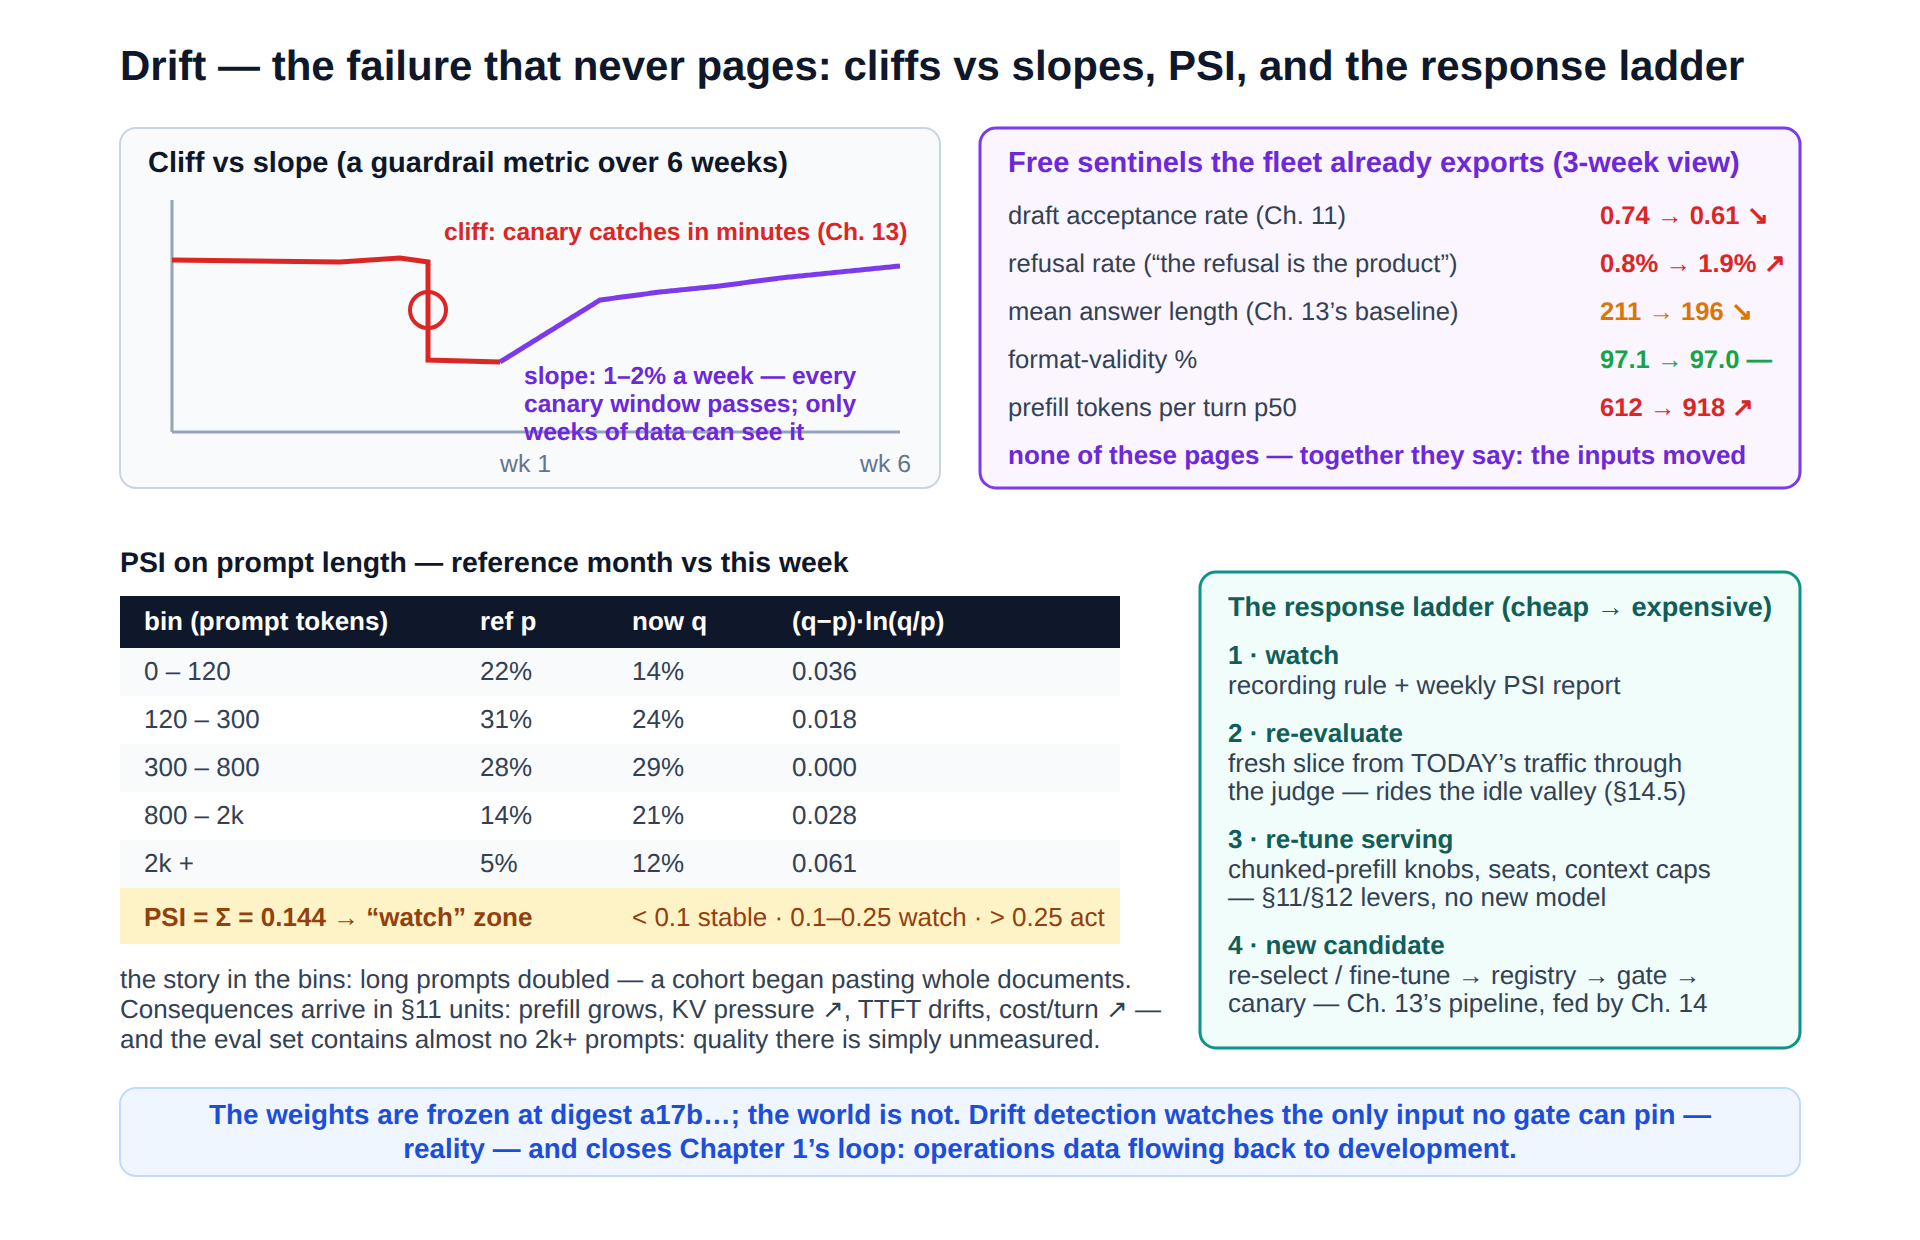
\includegraphics{figures/fig14-6_drift.png}}\\[3pt]
  \figcaption{Figure 14-6  Drift instrumentation. Top left: the cliff a canary catches versus the slope only weeks can see. Top right: sentinel metrics the fleet already exports, drifting in chorus. Bottom left: PSI on prompt length, computed by hand — 0.144, watch zone. Bottom right: the response ladder, cheap to expensive; rung 4 feeds Chapter 13’s pipeline and closes Chapter 1’s loop.}
\end{tbbfigure}

\subsection*{Sentinels you already export, and one number you can compute by hand}

Before building anything new, read Figure 14-6’s top-right panel: five lines the fleet has exported since Week 11, none of which pages, which \textit{together} say the inputs moved. \textbf{Draft acceptance rate} sliding 0.74 → 0.61 over three weeks is the answer to Chapter 11’s open question — \textit{what dashboard line detects speculative decoding’s silent failure mode?} — because acceptance is a live estimate of how well a tiny model predicts your traffic, which makes it a free, always-on distribution thermometer: when inputs wander from both models’ comfortable ground, the draft misses first, the speedup decays toward 1×, and the line falls — TPOT cost arriving before quality cost, an early-warning ordering you get for nothing. \textbf{Refusal rate} creeping 0.8\% → 1.9\% (the refusal is the product — but a \textit{rising} refusal share means the product is refusing people it used to serve, or the people changed). \textbf{Mean answer length} re-centering off Chapter 13’s 211-token baseline. \textbf{Format-validity} flat — a useful \textit{negative} sentinel, ruling drift-of-capability out even as drift-of-inputs shows. And \textbf{prefill tokens p50} up 612 → 918, the loudest line of the five and the one with immediate §11 consequences: longer prompts mean more KV per admit, more preemptions (the PreemptionSurge ticket in Table 14-2 is often drift announcing itself through the capacity plane), TTFT sliding toward the SLO line for purely arithmetical reasons. Sentinels are cheap correlation, not proof; when the chorus moves, you reach for a real distribution test.

The industry’s workhorse is the \textbf{Population Stability Index}, and its virtue is that you can compute it on a napkin, which means you can \textit{audit} it when a vendor dashboard waves it at you. Bin a feature over a \textbf{reference window} (the month around your last gate run — the world your eval set believes in); measure this week’s share per bin; then PSI = Σ (qᵢ − pᵢ) · ln(qᵢ/pᵢ) — each term positive wherever a bin grew or shrank, weighting relative change by absolute movement. Figure 14-6’s worked table runs it on prompt length: the 2k+ bin more than doubling (5\% → 12\%) contributes 0.061 all by itself, total \textbf{PSI = 0.144} — inside the conventional bands (< 0.1 quiet; 0.1–0.25 watch; > 0.25 act) that practitioners inherited from credit-scoring, where this index spent decades watching loan applicants drift. Two disciplines keep PSI honest: bin on the \textit{reference} quantiles (equal-mass bins, so the test has power everywhere the old world had mass), and run it per feature — length, language, route, hour-of-day — because a total that stays quiet can hide two features drifting in opposite directions. For semantics beyond hand-binnable features, the same recipe runs on \textbf{embeddings}: nightly mean-cosine distance from this week’s prompt-embedding centroid to the reference centroid, with the reference vectors stored beside the eval set in the registry (lineage for the \textit{measuring stick}, not just the model). And for the statistically fastidious, the Kolmogorov–Smirnov test replaces the binning with a supremum over CDFs — better calibrated p-values, less interpretable per-bin story; the course teaches PSI because the \textit{story in the bins} (“a cohort began pasting documents”) is the part an engineer can act on.

\subsection*{The response ladder — and who pays for the judge}

Detection without a decided response is a hobby, so the lab’s drift job ends every report with a rung from Figure 14-6’s ladder. \textbf{Rung 1, watch}: PSI in the watch band with sentinels quiet — annotate, keep the weekly cadence, do nothing (most weeks; drift work is mostly the discipline of not overreacting). \textbf{Rung 2, re-evaluate}: sample a fresh slice from \textit{this week’s} traffic, run it through the gate’s rubric — including the LLM-as-judge scoring the un-labelable qualities — and compare against the frozen eval set’s verdict. This is the rung that catches concept drift and eval staleness, and its economics close a loop from Chapter 12: judging 0.2\% of \textasciitilde{}9.5 M monthly turns at \textasciitilde{}1,600 tokens each is \textasciitilde{}30 M tokens a month of judge inference, which would be real money at API prices — but the committed-use floor bought 3.1 B tokens of capacity and traffic uses 2.0 B, so the judge runs \textit{inside the valley}, on capacity already paid for, at 3 a.m. beside Chapter 13’s Lane-3 nightly evals. Samuel Insull filled his overnight troughs with ice houses; you fill yours with quality control. Marginal cost: approximately zero, and the ledger stays at \$900. \textbf{Rung 3, re-tune serving}: when the drift is arithmetical (longer prompts), the levers are §11/§12’s, not the model’s — chunked-prefill knobs, seat counts, context caps, maybe the autoscaler’s target — a repricing, not a retraining. \textbf{Rung 4, new candidate}: when rung 2 shows quality genuinely off on the new world, the fix re-enters at the top of Chapter 13’s pipeline — new eval slices first (measure the world before chasing it), then fine-tune or re-select, registry, gate, canary, promotion. Note what that sentence \textit{is}: operations data flowing back to development — Chapter 1’s four-stage cycle, closed by the last chapter of the machinery. The drift report that triggered it is filed on the registry entry it dethrones, so the next incident reviewer reads why v9 retired, in evidence, not folklore.

\begin{terminalbox}
\begin{Verbatim}[breaklines=true,breakanywhere=true,fontsize=\small,formatcom=\color{tbbtermfg},codes=\tbbcodeactive]
$ kubectl logs job/drift-nightly | tail -18
drift-report 2026-XX-XX  ref=2026-XX (gate window for v9-int4)
  inputs:
    prompt_len   PSI 0.144  WATCH   (2k+ bin: 5% -> 12%)
    language     PSI 0.031  ok
    route_mix    PSI 0.008  ok
    embedding    d_cos 0.041 vs ref  ok (threshold 0.10)
  sentinels (21-day trend):
    accept_rate  0.74 -> 0.61   FALLING    refusal  0.8% -> 1.9%  RISING
    ans_len p50  211  -> 196    drifting   fmt_valid 97.1 -> 97.0  ok
    prefill p50  612  -> 918    RISING
  verdict: WATCH -> escalate rung 2 (fresh-slice eval tonight)
  actions:
    - queued: eval-fresh-slice (n=2000, stratified by length bin)
    - note: filed on registry entry chat/v9-int4 (drift/2026-XX-XX)
    - capacity: KV headroom check vs prefill p50 918 -> §11 sizing
  next run: tomorrow 03:10 (rides the valley, after lane-3 evals)
\end{Verbatim}
\end{terminalbox}
\figcaption{Transcript 14-5  The nightly drift job’s report — a dated, versioned artifact, not a dashboard vibe. PSI per feature with the story bin named; sentinels as trends; a verdict that is a LADDER RUNG; actions that are queue entries and registry notes. Slopes get reviews, not pages: nothing here wakes anyone, and everything here is read weekly, on purpose, in daylight.}

One closing distinction keeps teams out of a classic trap: \textbf{drift monitoring is not anomaly detection.} The instruments in this section compare \textit{windows to references} on schedule; they are slow, deliberate, and reviewed by humans — because the failure they hunt is slow, deliberate, and (for now) beyond automation to fix. Resist the vendor pitch of an ML system that watches your ML system and pages on “anomalies”: it re-imports the hospital ward through the back door, with false positives whose investigation cost lands on the same on-call this chapter just taught you to protect. The division of labor that works: \textbf{pages for cliffs} (§14.4, seconds-to-minutes, fully automated), \textbf{reviews for slopes} (this section, weeks, human-in-the-loop), and a calendar entry — not an alert — as the delivery mechanism for the weekly drift report. The most reliable drift detector ever deployed remains a senior engineer reading Transcript 14-5 with coffee, every Monday, asking Chapter 7’s oldest question: \textit{is the promise still the right promise?} — because the SLO itself drifts (a student fleet’s 500 ms mattered when rivals answered in 5 s; the bar moves), and no PSI computes that.

\begin{calloutbox}{tbbpurple}{tbbpurplefill}
{\normalsize\bfseries\color{tbbpurple}Think About It}\par\vspace{3pt}
\begin{tbbitemize}
  \item For each — (a) prompts shift from questions to pasted documents, (b) a national election changes  “current events” answers, (c) exam season doubles proof-checking requests — classify the drift type, name the FIRST instrument in this section to move, and pick the response rung. Which of the three could a perfect canary have caught at deploy time? (Trick question — say why.)
  \item PSI = 0.144 with equal-mass 5-bin binning. Recompute the same shift with 2 bins (0–300, 300+) and show the index shrinks — then state the general lesson about binning power, and why the reference quantiles (not this week’s) must define the bins.
  \item Acceptance rate is a “free” drift thermometer — but it confounds two causes (input shift vs. a draft-model update). Design the one-line registry check that disambiguates, and explain why the sentinel panel still earns its place even confounded.
  \item The judge rides the idle valley at \textasciitilde{}zero marginal cost. A teammate proposes 10× sampling (2\% of turns) “since it’s free.” Find the two places the free lunch ends (valley depth in tokens; judge-vs-serving contention at the 19:00 shoulder — Ch. 12’s staircase), and compute roughly where the ceiling is.
\end{tbbitemize}
\end{calloutbox}

\section{Lab: Mission Control — Build It, Then Break It Twice}

The syllabus promises “서빙 대시보드 구축과 알람 설정” — build the serving dashboard, wire the alarms — and this lab delivers both, then adds the step that separates instrument owners from instrument tourists: two staged failures, watched live on the panels you just built. Everything runs on the course’s standing lab rig (the T4 card, Qwen2.5-1.5B under vLLM — Week 11’s server, still warm) plus the classifier pair from Weeks 9–10; the absolute numbers will differ from the fleet’s, and per the course’s oldest rule that is fine — \textbf{you are graded on shapes and reasoning, never on matching the book’s constants.} Figure 14-7 is the map; six build steps, two drills, five deliverables.

\begin{tbbfigure}
  \adjustbox{max width=0.94\linewidth,max totalheight=0.46\textheight}{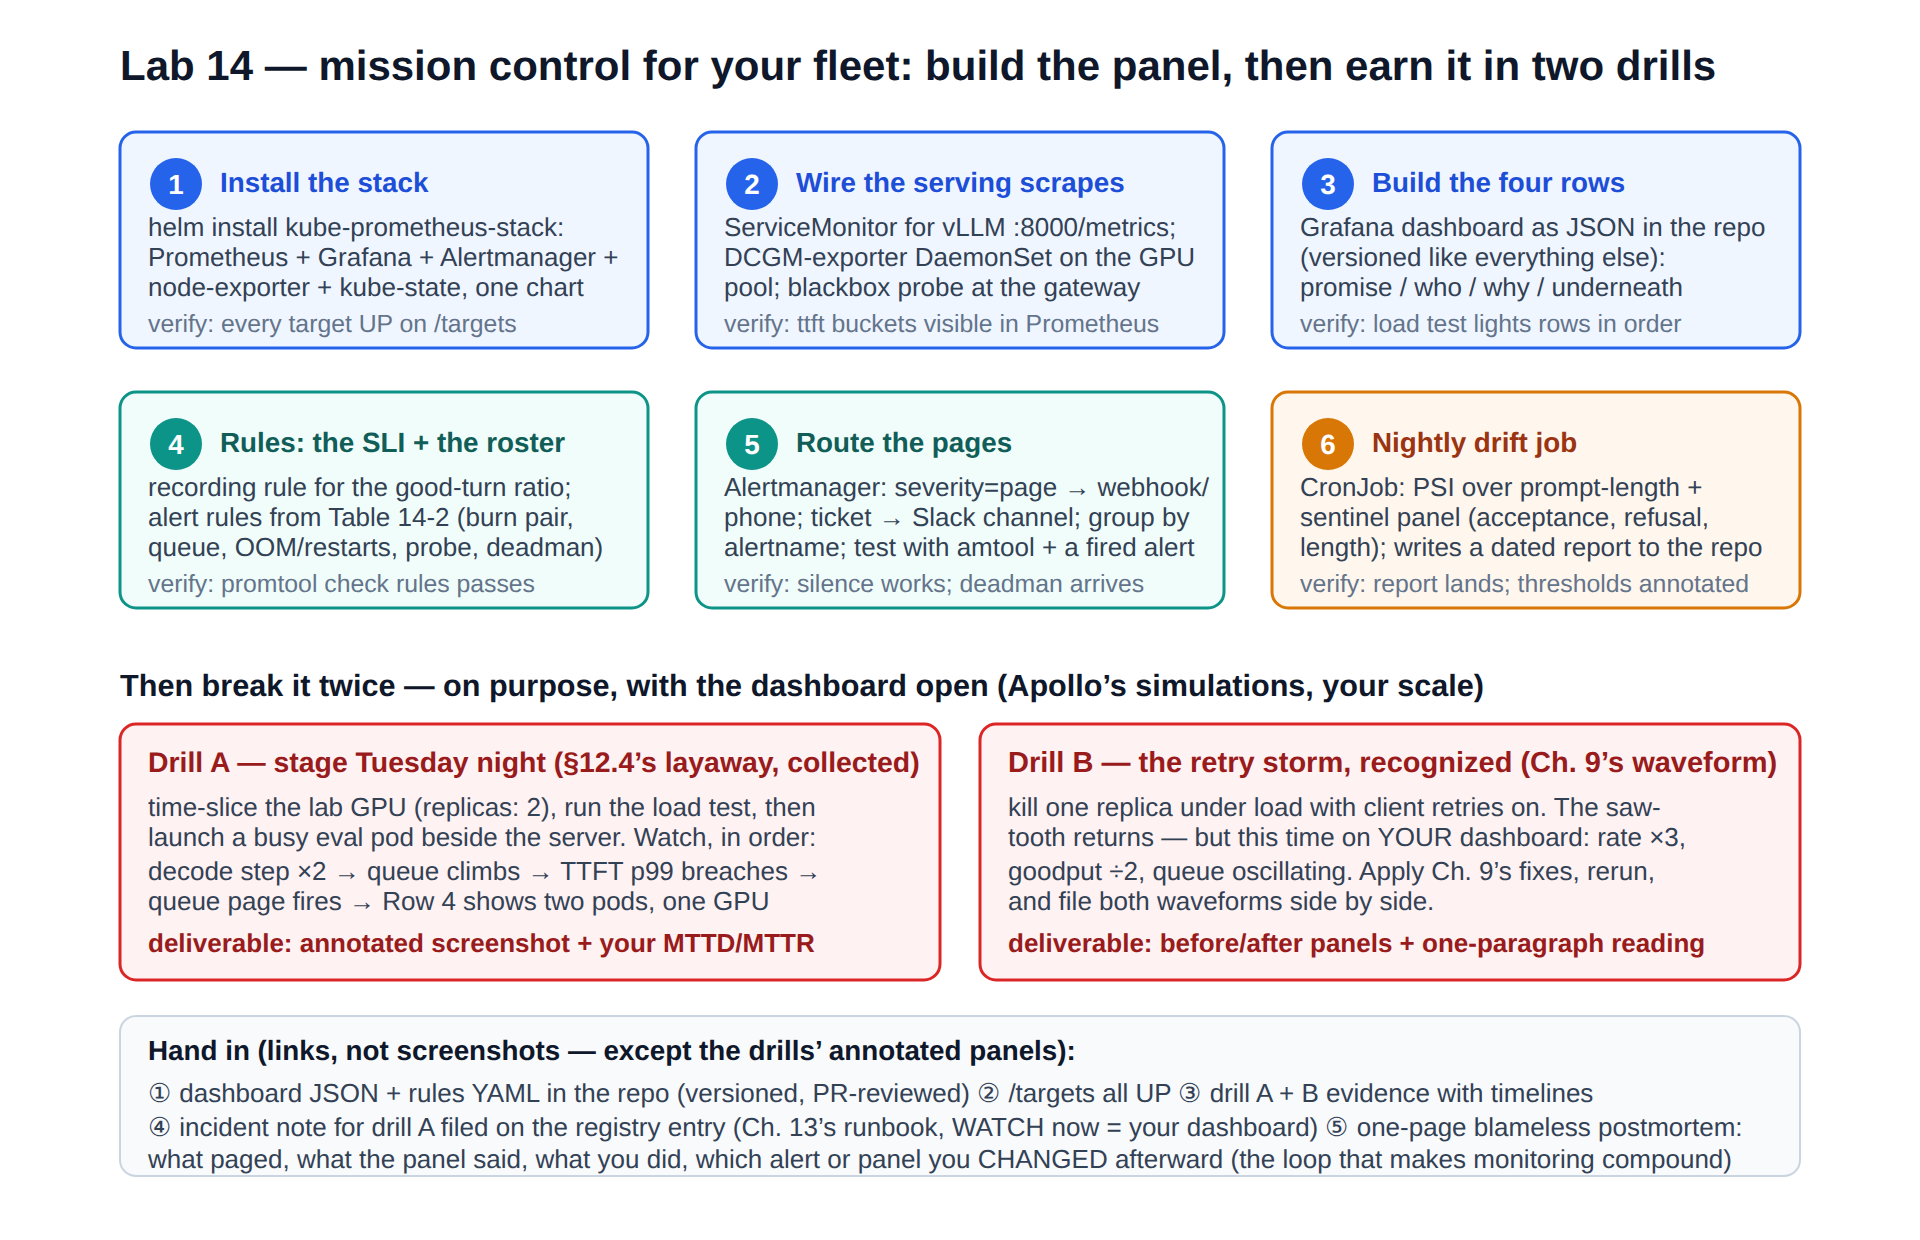
\includegraphics{figures/fig14-7_lab.png}}\\[3pt]
  \figcaption{Figure 14-7  Lab 14. Steps 1–3 stand the stack up and draw the four rows; steps 4–5 arm the roster and route the pages; step 6 schedules the drift job. Then drill A re-stages Tuesday night (§12.4’s layaway, collected on your own hardware) and drill B replays Chapter 9’s retry storm — this time with instruments. Deliverables are links; the two annotated drill screenshots are the only images graders accept.}
\end{tbbfigure}

\textbf{Steps 1–3, stand it up.} Helm-install \code{kube-prometheus-stack} (one chart: Prometheus, Grafana, Alertmanager, node-exporter, kube-state-metrics) and verify every target UP on \code{/\allowbreak targets} before touching anything else — a scrape roll call is the lab’s first honest deliverable, and \code{up == 0} rows are your first debugging exercise (the usual suspects: a Service without the port name the ServiceMonitor matches, a namespace the selector misses). Wire the serving scrapes with two ServiceMonitors (engine \code{:8000/\allowbreak metrics}, classifier) plus the DCGM DaemonSet on the GPU node and the blackbox exporter with §14.4’s three probes. Then build the \textbf{four-row dashboard as JSON in the repo} — panels from Table 14-1, the SLO line drawn on every panel that measures a promise, the pods-per-UUID table on row 4, and captions that teach (“pinned-high is healthy”; “busy ≠ yours”). Sanity-check by running Week 11’s token-aware load test at three concurrency steps and watching the rows light \textit{in causal order} — row 3’s queue first, then row 1’s p99, then (if you push past the knee) row 2 telling you it is everyone, not someone. If the rows light out of order, a query is wrong; the dashboard is now testing itself.

\textbf{Steps 4–6, arm it.} Encode the SLI recording rule and Table 14-2’s roster — for the lab’s single-user reality, scale the queue threshold to your measured seat count (Transcript 11-5’s census, not the fleet’s 8) and confirm \code{promtool check rules} passes in CI (rules are release artifacts; the pipeline gates them like weights). Route pages to a phone-adjacent receiver (a webhook that pings your own device is fine) and tickets to a channel; prove the plumbing with \code{amtool} — fire a synthetic alert, watch it group, silence it, watch the silence hold — and stand up the dead man’s receiver \textit{outside the cluster} (the free tier of any heartbeat service, or a cron on a lab VM, suffices: the point is fate not shared). Schedule the drift CronJob at 03:10 with a reference window frozen to your Week 10 gate run; its first real report is due with the deliverables, WATCH verdicts and all. Then — the graded part — \textbf{break it twice.}

\begin{terminalbox}
\begin{Verbatim}[breaklines=true,breakanywhere=true,fontsize=\small,formatcom=\color{tbbtermfg},codes=\tbbcodeactive]
# drill A -- stage tuesday night against your own server (lab GPU, qwen-1.5b)
$ kubectl patch cm nvidia-device-plugin -p '{"data":{"config":"replicas: 2"}}'
$ locust -f loadtest.py --headless -u 24 &          # steady load, seats full
$ kubectl create job eval-burn --image=... -- python soak.py --busy
# watch, in order (screenshot each transition):
#   row 3: decode step p50 0.021 -> 0.044   <- the neighbor's tax
#   row 3: num_requests_waiting 0 -> 11     <- the queue is local
#   row 1: TTFT p99 0.28 -> 2.9s; SLI ratio dives
#   21:0X  PAGE QueueSustained (your phone buzzes; note the clock)
#   row 4: pods-per-UUID: your-gpu: 2 (qwen-srv, eval-burn)
$ kubectl delete job eval-burn && date              # note the clock again
#   queue drains; page auto-resolves. MTTD = page - patch. MTTR = delete - patch.

# drill B -- week 9's retry storm, now with instruments (classifier pair)
$ locust -f storm.py --headless -u 60 &   # client retries ON (the bad config)
$ kubectl delete pod classifier-1         # kill one of two under load
#   rows: req rate x3 (retries multiplying), goodput /2, queue sawtooth --
#   the waveform from week 9, on YOUR panels. now apply ch. 9's fixes
#   (retry connect-only, one layer, jitter, shed early) and re-run:
#   same kill, flat goodput, no storm. file both panels side by side.
\end{Verbatim}
\end{terminalbox}
\figcaption{Transcript 14-6  The two drills. Drill A collects §12.4’s layaway on your own hardware — the time-slice ConfigMap, a busy neighbor, and the exact panel sequence from Figure 14-4, with your phone as the pager and the wall clock as the grader. Drill B replays Chapter 9’s storm so that the waveform lives in your visual memory next to the panel that draws it — the “two Grafana screenshots” that chapter promised would matter at 2 a.m., finally taken.}

\textbf{What you hand in} (links, not screenshots — except the two annotated drill panels): the dashboard JSON and rules YAML in the repo with their PR history; the \code{/\allowbreak targets} roll call; drill A’s annotated timeline with \textit{your measured MTTD and MTTR} against Figure 14-1’s 12-and-8; drill B’s before/after storm panels with a one-paragraph reading; the drift job’s first report; and — the deliverable that ties the whole term together — \textbf{an incident note for drill A filed on your registry entry} using Chapter 13’s runbook (whose WATCH line now names your dashboard rows), plus a one-page blameless postmortem whose action-items section must contain at least one \textit{change to the monitoring itself}: a new alert, an edited threshold, a caption that will save the next 2 a.m. brain thirty seconds. That last requirement is the lab’s thesis in miniature: a monitoring stack is finished the way a garden is finished — never, and on purpose, one incident at a time.

\begin{calloutbox}{tbbamber}{tbbxFFFBEB}
{\normalsize\bfseries\color{tbbx92400E}Box 14-2  Grading rubric — Lab 14 (and the red flags that cost marks)}\par\vspace{3pt}
\begin{tbbitemize}
  \item \textbf{Stack + scrapes (20\%).} All targets UP with evidence; ServiceMonitors and exporters in the repo, not hand-applied. Red flag: a dashboard querying metrics whose targets show 0/N — panels of confident emptiness.
  \item \textbf{Dashboard design (25\%).} Four rows answering four questions in runbook order; SLO lines drawn; legal percentile aggregation everywhere (one avg-of-p99s anywhere on the board caps this criterion at half). Captions that teach.
  \item \textbf{Alarm roster (20\%).} Burn pair reading recording rules; queue page with sustain; causes ticketed, not paged; deadman verified end to end. Red flag: a roster that would page more than weekly under normal lab traffic — count it and say so.
  \item \textbf{Drills (25\%).} Both staged, both caught by YOUR alerts (not by watching), MTTD/MTTR measured and compared honestly; drill B shows the fix working, not just the failure failing. Red flag: screenshots without clocks.
  \item \textbf{The loop (10\%).} Incident note on the registry entry; postmortem with a monitoring-changing action item, shipped as a PR. This is the criterion that predicts who will run real fleets well.
\end{tbbitemize}
\end{calloutbox}

\begin{calloutbox}{tbbpurple}{tbbpurplefill}
{\normalsize\bfseries\color{tbbpurple}Think About It}\par\vspace{3pt}
\begin{tbbitemize}
  \item Drill A on a time-sliced T4 changes decode step by \textasciitilde{}2.1× but the classifier drill on CPU barely moves p50 while p99 triples (Transcript 12-4’s shape). Explain both from first principles — which resource each workload saturates, and why time-slicing taxes tails before medians.
  \item Your queue page threshold came from Transcript 11-5’s seat census. Week 12’s autoscaler now changes replica counts hourly. Propose the threshold expression that survives autoscaling (hint: per-pod gauge vs. fleet sum; which one did Table 14-2 choose and why), and name the failure mode of getting it backwards.
  \item During drill B’s BAD run, row 1’s SLI barely moved for the first 60 seconds while row 3 screamed. Reconcile with §14.4’s “symptoms page, causes ticket” — is a queue sawtooth a symptom or a cause during a retry storm, and what does your answer imply about the QueueSustained sustain window?
  \item The postmortem asks for a monitoring change. Argue which single change from drill A generalizes best to the project fleet: the pods-per-UUID ticket, a decode-step-vs-baseline ratio panel, or a per-pool time-slice-config expiry check in CI — and what class of future incident each choice fails to prevent.
\end{tbbitemize}
\end{calloutbox}

\namedsection{Summary}{The Chapter in Sixteen Points}

\qitem{1}{\textbf{Two nights, one thesis: at 2 a.m. you can only see what you graphed at 2 p.m.} Night one’s five checks all returned true answers to the wrong questions — probes measure aliveness, logs record confessions, means describe nobody, one pod is an anecdote, GPU util counts anyone. 85 bad minutes. Night two: 20, same brain, questions pre-asked.}

\qitem{2}{\textbf{Apollo is the syllabus in miniature.} Telemetry is designed in advance or does not exist (nobody ssh-es into a rocket, or a fleet); raw signal saves nothing — RECOGNIZED SIGNATURES do (SCE-to-AUX was a drill remembered); and the cheat sheet that saved the landing was written after a failed simulation. Instrument, rehearse, annotate.}

\qitem{3}{\textbf{Probes are reflexes; monitoring is memory} (Ch. 5’s line, cashed): a dashboard is memory, an alert is attention, a drift monitor is foresight. Observability is the property that lets you answer questions you did not predefine — Tuesday’s collision had no panel, and four generic rows answered it anyway.}

\qitem{4}{\textbf{Three pillars, priced by cost shape:} metrics (per-series, cheap, always-on — alerts live here), logs (per-event, the pod’s biography, shipped OFF the pod before it dies — Ch. 6 paid), traces (per-request, sampled, thin in a 3-hop course). Ch. 5’s entourage arrives: exporter and log shipper installed; mesh stays parked (one owner per concern).}

\qitem{5}{\textbf{A metric is name + labels + value + time; you pay per SERIES.} Labels answer “which one?” from bounded lists (pod, UUID, route); anything unbounded (user, request) belongs in logs. Cardinality is the memory wall of monitoring: one careless label multiplies 14k series a thousandfold.}

\qitem{6}{\textbf{Three shapes, one commandment.} Counters climb (rate() them, restart-proof); gauges read now (saturation’s shape); histograms exist because PERCENTILES DO NOT AVERAGE — bucket counters add across replicas, percentiles of the merged buckets are the only legal fleet p99. avg-of-p99s said 2.76 s; the truth was 9.08.}

\qitem{7}{\textbf{Pull, because absence must be a fact:} every scrape writes up\{pod\}, and a dead target leaves a tombstone instead of a silence. The lineage is Borgmon → Prometheus (SoundCloud 2012, CNCF project \#2 after Kubernetes) + Grafana (a 2014 Kibana fork); recording rules precompute the SLI and ship through Ch. 13’s pipeline — rules are release artifacts.}

\qitem{8}{\textbf{The exporter menagerie is the course, re-traversed:} node-exporter (Ch. 2’s machine), cAdvisor reading cgroup files from outside — honest mounts (Ch. 3, incl. memory.events’ oom\_kill and the memory.high tripwire, now graphable), kube-state (Ch. 5’s alert list: restarts, OOMKilled, endpoints, rollout state), DCGM (nvidia-smi industrialized, per-UUID, joined to pods), the engine’s /metrics (Ch. 11’s lines), blackbox (Ch. 6’s door, probed from outside).}

\qitem{9}{\textbf{GPU “utilization” is an occupancy duty cycle: busy ≠ yours ≠ efficient.} A memory-bound decode reads 90\%+ at a tenth of the ALUs; two tenants both read \textasciitilde{}100\%; nothing says whose. Saturation signals lead (queue, preemptions, DRAM activity); utilization lags and lies. USE for resources, RED for services; the queue is the master saturation gauge.}

\qitem{10}{\textbf{The four-row dashboard: promise → who → why → underneath.} Row 1 is the SLO sentence as panels (budget, burn, legal p99, per-stream pace) and the only row that pages; Row 2 forks everyone-vs-someone (RED per replica); Row 3 is the engine’s why (queue, KV pinned-high-healthy, decode pace, preemptions — Ch. 9’s queue/compute split kept); Row 4 is the substrate (DCGM per UUID, pods-per-GPU, autoscaler posture).}

\qitem{11}{\textbf{Symptoms page; causes ticket.} Symptoms are few, real, and complete (novel failures still surface in the SLI — the collision proved it); causes are legion, cheap, and often harmless. Hospitals taught the price (85–99\% of alarms need no action; alarm fatigue kills). Every page: actionable, urgent, real.}

\qitem{12}{\textbf{The SLO sentence compiles to burn rates.} p99 ≤ 500 ms ≡ 99\% of turns good → SLI ratio → budget = 1\% × \textasciitilde{}9.5M turns ≈ 95k bad turns/30 d. Burn = bad-fraction ÷ 0.01; the multiwindow policy (14.4×/1 h∧5 m page, 6×/6 h page, 3×/1× ticket): long window = skepticism, short = forgiveness. Fast paths on leading symptoms (the queue) are allowed.}

\qitem{13}{\textbf{Stand outside every layer that can say no:} three synthetic probes (door / answer / stream), each outside the layer it indicts, paging on persistence not existence — Exhibit 14-A’s green /health was probe one alone. The Watchdog fires ALWAYS so its silence pages via a receiver that shares no fate with the cluster: the dead man’s switch watches the watcher.}

\qitem{14}{\textbf{The human loop makes monitoring compound:} pages carry runbooks whose WATCH step names dashboard rows; incidents end in blameless postmortems (mechanisms, not names) whose action items CHANGE THE MONITORING — every fire leaves a smoke detector. Notes file on the registry entry (Ch. 10’s reviewer, reading at last); MTTD/MTTR grade the loop and close DORA’s fourth key. The stack costs \textasciitilde{}\$23/mo — the ledger closes at exactly \$900.}

\qitem{15}{\textbf{Drift is the failure that never pages: canaries catch cliffs; drift monitors catch slopes.} Taxonomy by response: data drift (inputs moved — serving arithmetic and eval coverage break first), concept drift (right answers moved — only fresh-world eval sees it), prior shift (task mix moved — re-baseline the guardrails), and eval-set staleness (the yardstick drifts too — resample quarterly). Sentinels come free (acceptance — Ch. 11’s question answered — refusal, length, prefill p50). PSI is computable by hand — 0.144, watch zone — and slopes get REVIEWS, not pages.}

\qitem{16}{\textbf{The response ladder prices the reaction:} watch → re-evaluate on a fresh slice (the judge rides the idle valley — Insull’s ice house, \$0 marginal on the committed floor) → re-tune serving → new candidate through Ch. 13’s registry→gate→canary — operations data flowing back to development, Chapter 1’s cycle closed. And the Monday question no PSI computes: is the promise still the right promise?}

\namedsection{Exercises}{}

\subsection*{A. Multiple choice}

\qitem{1}{Night one’s five checks (probes, logs, mean, one pod’s p99, nvidia-smi) all “passed” during a real outage because:}

\begin{tbboptions}
  \item ① The tools were misconfigured        ② Each answers a different question than the SLO asks — aliveness, confessions, central tendency, an anecdote, occupancy — and none computes the promise
  \item ③ The incident was too short to observe        ④ The fleet lacked enough replicas
\end{tbboptions}

\qitem{2}{Averaging four per-replica p99s produced 2.76 s against a true fleet p99 of 9.08 s. The root error:}

\begin{tbboptions}
  \item ① The window was too short        ② Percentiles are not linear — only the merged distribution’s quantile is meaningful, and only bucket COUNTERS add across replicas
  \item ③ rate() was omitted        ④ The buckets were misaligned with the SLO
\end{tbboptions}

\qitem{3}{DCGM\_FI\_DEV\_GPU\_UTIL reads 93\%. What is actually known:}

\begin{tbboptions}
  \item ① The GPU is 93\% of the way to saturation        ② Your pod is using 93\% of the FLOPs
  \item ③ For 93\% of recent time, at least one kernel — from ANYONE — was resident: occupancy duty cycle, silent on headroom, efficiency, and ownership        ④ 7\% of capacity is available for a neighbor
\end{tbboptions}

\qitem{4}{Garman’s “GO if it doesn’t recur too often” is, in this chapter’s machinery:}

\begin{tbboptions}
  \item ① A silence        ② The severity ladder        ③ A dead man’s switch        ④ Rate-and-persistence alerting — for:, sustained windows, paired burn windows — paging on recurrence, never on existence
\end{tbboptions}

\qitem{5}{Burn rate 24× on a 99\% / 30-day SLO means:}

\begin{tbboptions}
  \item ① 24\% of requests are failing the SLO threshold — and at that pace the month’s budget is gone in \textasciitilde{}30 h (30 d ÷ 24)        ② The SLO is 24× too strict
  \item ③ p99 is 24× the threshold        ④ The pager will fire 24 times
\end{tbboptions}

\qitem{6}{The burn-rate page guarantees completeness; the QueueSustained page exists anyway because:}

\begin{tbboptions}
  \item ① Burn rules are unreliable        ② Queues are causes and causes deserve pages
  \item ③ At 24× burn the 1-hour window needs \textasciitilde{}35 minutes to cross 14.4× — the queue is the LEADING symptom, and fast paths are allowed for symptoms        ④ Alertmanager cannot route two pages
\end{tbboptions}

\qitem{7}{The Watchdog alert evaluates vector(1) — it fires forever — because:}

\begin{tbboptions}
  \item ① It keeps the pager warm        ② Its ABSENCE at an external receiver is the alarm: if the heartbeat stops, the monitoring stack itself is down — the dead man’s switch
  \item ③ Prometheus requires one active alert        ④ It measures alert latency
\end{tbboptions}

\qitem{8}{The nightly job reports prompt-length PSI = 0.144 with sentinels drifting in agreement. Correct response:}

\begin{tbboptions}
  \item ① Page the on-call        ② Retrain immediately        ③ Watch zone (0.1–0.25): weekly review, escalate rung 2 — a fresh-slice evaluation — because slopes get reviews, not pages        ④ Raise the SLO threshold
\end{tbboptions}

\subsection*{B. Short answer}

\qitem{1}{Write the PromQL for the fleet’s TTFT p99 and name what each of the three layers (rate, sum by le, histogram\_quantile) contributes — including why the innermost one is restart-proof.}

\qitem{2}{KV-cache usage is pinned at 96\% and nothing alarms; num\_requests\_waiting sits at 9 for six minutes and a human wakes up. Justify both designs from Chapter 11’s architecture — what is each gauge measuring, and which one is demand exceeding seats?}

\qitem{3}{Specify the three synthetic probes (path, frequency, alert condition) and, for each, the layer it must stand OUTSIDE of to be a witness rather than a mirror — mapping each to the Chapter 6 failure class (503 / 504 / stream-cut) it catches first.}

\qitem{4}{Chapter 7’s 99.9\% bought 43 minutes; this chapter’s 99\% bought 95,000 turns. Explain why the request-based unit prices the diurnal wave correctly where the time-based one cannot — what does a bad minute cost at 03:00 versus 21:30 in each accounting?}

\qitem{5}{Classify as page or ticket, with one clause each: (a) endpoints ready = 0; (b) pods-per-prod-UUID = 2; (c) probe\_success 3× consecutive fail; (d) OOMKilled seen once on one replica; (e) burn 6× over 6 h; (f) preemption rate 0.8/s for 10 min.}

\qitem{6}{Explain the acceptance-rate sentinel: why a falling draft-acceptance line is an input-distribution thermometer, what cost arrives before what cost, the confound that can fake the signal, and the registry query that disambiguates.}

\subsection*{C. Essay}

\qitem{1}{Write Tuesday’s blameless postmortem: minute-level timeline (both alerts, the walk, the evict), impact in bad user-minutes with the night-one counterfactual (20 vs. 85), root cause as MECHANISMS (the stale time-slice ConfigMap; the missing pods-per-UUID policy — never a name), and three action items with owners — at least one changing the monitoring itself. Close with the paragraph most postmortems omit: what this incident does NOT justify building, and why.}

\qitem{2}{Design the complete paging policy for your project fleet under an explicit alarm-fatigue budget of two pages per month at steady state. Roster with severities and windows justified from YOUR measured traffic (seat counts, arrival rates), the deadman’s external receiver, grouping/inhibition rules — and the section auditors read first: which failure classes you consciously demoted to tickets, and the user-pain each demotion accepts.}

\qitem{3}{“Monitoring is the canary’s analysis window made permanent.” Trace answer-length from Friday’s bug (Ch. 13) through the canary guardrail, the recording rule, and the drift sentinel: for each timescale give the window, the threshold style (hard vs. baseline-relative vs. reference-distribution), the audience, and the response — then argue why the SAME number serves all three instruments, and what that implies about which metrics deserve to exist at all.}

\qitem{4}{The observer-cost essay: price the monitoring stack honestly (the \$23 line, the TSDB napkin, the judge’s valley ride, the on-call’s attention as the scarcest resource) and identify where observability’s marginal value crosses its marginal cost for a fleet of this size. Then resolve Chapter 7’s 2 a.m. essay with this chapter’s instruments — budget panel, pre-agreed loosening clause, runbook — and defend or attack: “boring operations is the correct terminal state of this entire course, and the \$23 was the cheapest line on the bill.”}

\namedsection{Answers and Commentary}{}

\subsection*{A. Multiple choice}

\qitem{1}{\textbf{②} Five honest instruments, zero assembly: the SLO’s own definition of “fine” (the SLI) was computed nowhere, decomposed nowhere. Row 1 replaces all five for the promise; rows 2–4 replace the search. (§14.1)}

\qitem{2}{\textbf{②} The mean of tails is a fiction (a 9.8 s replica and three 0.4 s replicas average to a latency nobody had); merged buckets ARE the fleet distribution. This is Ch. 7’s fourth grammar rule with tooling to enforce it. (§14.2)}

\qitem{3}{\textbf{③} Duty cycle of any-kernel-resident: a memory-bound decode loop pins it high while starving ALUs; a neighbor’s kernels count too. Headroom lives in saturation and PROF\_* metrics; ownership lives in the pods-per-UUID join. (§14.2)}

\qitem{4}{\textbf{④} The 1202 was intermittent AND guidance still flew — a rate condition plus a symptom check, decided in writing before the descent. for:, sustained averages, and paired windows are the same judgment, mechanized. (§14.4)}

\qitem{5}{\textbf{①} Burn = bad-fraction ÷ (1 − SLO) = 0.24 ÷ 0.01; time-to-empty = 30 d ÷ burn. The framing to keep: burn is a SPEND RATE on a budget, which is what makes multi-speed policies coherent. (§14.4)}

\qitem{6}{\textbf{③} The long window’s skepticism costs latency (35 min at 24×); capacity-shaped pain announces itself queue-first (Ch. 7’s knee, Ch. 11’s admission line), so the symptom fast-path pages in \textasciitilde{}7. Both are symptoms; the purist’s objection is answered in the think box. (§14.4)}

\qitem{7}{\textbf{②} Silence-as-alarm inverts the failure mode: a dead Prometheus cannot page about itself, so the page must come from something it CANNOT kill — external receiver, no shared fate (region, billing, webhook chain audited separately). (§14.4)}

\qitem{8}{\textbf{③} Drift is a slope; paging on slopes re-imports alarm fatigue. The watch verdict schedules rung 2 (fresh-slice eval, riding the valley), files the report on the registry entry, and keeps humans in the loop at review cadence. (§14.5)}

\subsection*{B. Short answer}

\qitem{1}{histogram\_quantile(0.99, sum by (le) (rate(vllm:time\_to\_first\_token\_seconds\_bucket[5m]))). rate() turns cumulative bucket counters into per-second flows and bridges counter resets (pod rebirth shows as a reset, detected and compensated — Ch. 5’s reconciliation would otherwise poison every graph); sum by (le) merges replicas while preserving bucket edges — the only legal cross-replica aggregation; histogram\_quantile interpolates the quantile inside the winning bucket, ±bucket width. (§14.2)}

\qitem{2}{The KV pool is a cache-shaped ALLOCATION: PagedAttention’s design goal is a full pool (seats amortizing the weight stream — pinned-high is the machine earning rent; Ch. 3’s page-cache lesson, GPU edition). The queue is ADMISSION: sustained waiting means arrivals exceed seat throughput — demand past capacity, users already paying TTFT for it. One gauge full = working; the other gauge nonzero-sustained = failing. (§14.2, Ch. 11)}

\qitem{3}{Door: HTTPS GET /v1/models from outside the LB, 30 s, page on 3× fail — catches 503-class (TLS, target health, routing) because it stands outside the perimeter the fleet cannot see. Answer: 1-token completion, 60 s, 10 s timeout — catches 504/hang past the door (admission, engine) from outside the gateway. Stream: short streamed completion, first token ≤ 2 s and final chunk intact, 5 min — catches stream-cut from outside the idle-timeout layer (Table 6-3’s third row). Shared rule: a probe inside the layer it checks is a mirror. (§14.4, Ch. 6)}

\qitem{4}{Time-based budgets price all minutes equally; the staircase does not — a 03:00 minute carries \textasciitilde{}⅓ the turns of a 21:30 minute (Ch. 12’s wave). Request-based budgets spend in USER units: Tuesday’s 20 minutes at peak cost \textasciitilde{}24\% × 23/s × 1,200 s ≈ 6.6k bad turns (7\% of the month), which time-accounting would book identically at 03:00 despite hurting a third as many people. Page urgency should track people hurt; hence turns. (§14.4)}

\qitem{5}{(a) PAGE — nobody to route to, every user sees 503 now. (b) ticket — cause; harmless on dev, damning context once a symptom fires. (c) PAGE — the door is refusing real users, from the only vantage that can tell. (d) ticket — one OOM is Ch. 5’s buffered incident; page only if fleet-wide (systemic limit error). (e) PAGE — the slow-bleed pairing exists precisely because 6× over 6 h never trips the fast rule. (f) ticket — pool pressure, often drift arriving; investigate in daylight (§14.5). (§14.4)}

\qitem{6}{Acceptance estimates how well the tiny draft predicts live traffic — a distribution-match meter updated every request, free. When inputs wander, the draft misses first: TPOT decays toward the undrafted floor (a COST regression) before quality visibly moves — early warning, correct ordering. Confound: a draft-model or engine update also moves acceptance; disambiguate with registry lineage (did the release triple’s digests change on the trend’s start date?). Confounded or not, it belongs on the sentinel panel: a chorus, not a verdict. (§14.5, Ch. 11)}

\subsection*{C. Essay (grading points)}

\qitem{1}{Look for: dual-alert timeline with the ticket’s 11-minute head start noticed; impact in turns AND user-minutes with the counterfactual (85) argued, not asserted; mechanisms named (stale ConfigMap with no owner/expiry; missing placement policy) with the engineer explicitly de-blamed; three actions of different KINDS (alert promoted to policy, CI expiry check, caption edit) each owned and dated. The “won’t build” paragraph separates bands: e.g., rejecting per-pod anti-affinity everywhere (kills §12.4’s legitimate dev-pool sharing) or a bespoke anomaly detector (§14.5’s trap) — priced, not vibed. (§§14.1–14.4)}

\qitem{2}{The budget forces real choices; reward rosters that COUNT (expected fires/month per rule from measured traffic, summed, compared to 2). Musts: burn pair + one leading symptom + door probe as the page core; deadman external; grouping so one incident is one page; inhibition that never touches the Watchdog. The demotions section is the essay’s heart — e.g., single-replica OOM to tickets accepts one restart-lap of latency (§3.6/§5.6 arithmetic); preemption surges to tickets accepts a slow TTFT drift until review. Full credit requires the accepted pain QUANTIFIED. (§14.4)}

\qitem{3}{The trace: Friday — 211→54 in minutes, hard 30\% guardrail, audience = the canary controller, response = auto-retreat (Ch. 13). Recording rule — 5-min windows forever, threshold vs. rolling baseline, audience = Row 2/on-call, response = investigate. Drift sentinel — 21-day trend vs. gate-window reference, PSI-style bands, audience = the Monday review, response = the ladder. Strong essays name the invariant: one number, three WINDOWS, three response speeds — and conclude that metrics worth exporting are exactly those that can serve multiple timescales (guardrails earned permanence; vanity metrics never acquire a second instrument). (§§14.3–14.5, Ch. 13)}

\qitem{4}{The honest ledger: \$23 stack + \textasciitilde{}\$0 judge (valley) + TSDB growth bounded by retention — against the on-call’s attention as the binding constraint (alarm fatigue is a COST even when the cloud bill isn’t). The crossing: more panels/alerts stops paying when marginal signal is sub-actionable — Box 14-1’s sins are the symptoms of exceeding it. The 2 a.m. replay must cite Row 1’s budget graph + the Week 7 document’s pre-agreed clause and land on “arithmetic plus a signature.” On the thesis: strong defenses trace boring = automated + versioned + gradual + reversible (Ch. 13) + OBSERVED (Ch. 14) and note the \$23 bought the night-two delta (65 user-minutes, first incident); strong attacks note boring is a property of operations, not of the work — the interesting problems moved up the stack (drift, evals, product). Either stance with consistent arithmetic earns the top band. (§14.4, chapter-wide)}

\namedsection{Further Reading}{}

Entries tagged \textbf{[This week]} support the lab directly; \textbf{[Wk N]} marks material that pays off later.

\begin{tbbitemize}
  \item \textbf{[This week] Google SRE Book, ch. 6 “Monitoring Distributed Systems” + SRE Workbook, ch. 5 “Alerting on SLOs”} — the four golden signals, symptom/cause doctrine, and the exact multiwindow multi-burn-rate policy Table 14-2 adopts (read the Workbook chapter with Figure 14-5 beside it; the numbers match on purpose).
  \item \textbf{[This week] Rob Ewaschuk, “My Philosophy on Alerting”} — the short document that seeded “pages must be actionable, urgent, real”; the origin of symptoms-page-causes-ticket in something like its modern form. Twenty minutes, career-long returns.
  \item \textbf{[This week] Prometheus documentation: “Histograms and summaries” + “Querying basics”; and the Robust Perception blog} — bucket design, why summaries don’t aggregate (the sharp edge §14.2 sanded), rate() subtleties; Brian Brazil’s blog is the trade’s accumulated folklore, written down.
  \item \textbf{[This week] kube-prometheus-stack chart docs + Grafana dashboard best practices + NVIDIA DCGM-exporter README} — the lab’s three install surfaces; the DCGM README’s metric table is where util’s fine print and the PROF\_* family live, and its pod-mapping section powers Row 4’s smoking gun.
  \item \textbf{D. Sculley et al., “Hidden Technical Debt in Machine Learning Systems” (NeurIPS 2015)} — the paper that named what §14.5 monitors: entanglement, feedback loops, and the world changing under a frozen model. Read the “monitoring and testing” section last — it is this chapter in four paragraphs, a decade early.
  \item \textbf{Chip Huyen, Designing Machine Learning Systems, ch. 8 (“Data Distribution Shifts and Monitoring”)} — the drift taxonomy at book depth, with the estimation subtleties (windows, references, seasonality) the course’s PSI treatment compresses.
  \item \textbf{The Joint Commission, Sentinel Event Alert \#50: “Medical device alarm safety in hospitals” (2013)} — read a hospital-safety bulletin as an engineer and find every §14.4 principle stated in lives instead of nines; the citation behind “85–99\%” and the strongest argument you will ever have against a noisy roster.
  \item \textbf{[Fun] “13 Minutes to the Moon” (BBC World Service podcast, season 1)} — the 1202 alarm episode features Garman, Bales, and Hamilton telling §14.4’s opening story themselves; then find Sy Liebergot’s telling of Apollo 12’s SCE-to-AUX for §14.1’s. Mission control audio holds up as operations education disguised as history.
\end{tbbitemize}

\vspace{5.0pt}

\begin{calloutbox}{tbbblue}{tbbbluefill}
{\normalsize\bfseries\color{tbbblue}Next week — Week 15: Demo Day — the flight, flown}\par\vspace{3pt}
Fifteen weeks ago this course began with thirty seconds of silence and a spinning cursor — Exhibit A, a model that worked and a service that didn’t. Week 15 is the other bookend: 팀 프로젝트 발표와 시연 — your team, live, demonstrating the thing this book has been assembling one layer at a time. The machinery chapters are done; what remains is the evidence. The strongest demos will be the most boring ones: traffic flowing through a gateway with a key and a quota (Ch. 6), answered inside the SLO sentence your team re-negotiated in Week 11, on a fleet whose bill closes at a number you chose on purpose (\$4,762 → \$877 → \$900, every step explained), deployed by a pipeline that has refused a bad release in front of witnesses (Ch. 13) — all of it watched, during the demo itself, on the four-row dashboard you built this week, so that if anything breaks mid-presentation you diagnose it live, which is not the failure case but the highest form of full marks. Bring the registry lineage, the gate reports, the two red runs, the drill postmortem, the drift report, the final ledger. The demo is thirty minutes; the artifact trail is the grade. Fly the mission.
\end{calloutbox}
